
\documentclass[letter]{article}
\usepackage[utf8]{inputenc}
\usepackage[margin=1in]{geometry}
\usepackage{tikz}
\usepackage{ulem}
\usepackage{graphics}
\usepackage{sidecap}
\usepackage{wrapfig}
\usepackage[toc,page]{appendix}
\usepackage{caption}
\usepackage{amssymb}
\usepackage{amsmath}
\usepackage{algorithmicx}
\usepackage{algpseudocode}

\usepackage{url,graphicx,tabularx,array,geometry,amsmath,tikz}
\usepackage{algorithm}% http://ctan.org/pkg/algorithms
\usepackage{algpseudocode}% http://ctan.org/pkg/algorithmicx
\usepackage{listings}
\usetikzlibrary{arrows}
\newenvironment{myindentpar}[1]% %indent whole paragraph when needed
 {\begin{list}{}%
         {\setlength{\leftmargin}{#1}}%
         \item[]%
 }
 {\end{list}}

\usepackage{hyperref}
\usepackage{parskip}

\hypersetup{
    colorlinks,%
    citecolor=black,%
    filecolor=black,%
    linkcolor=black,%
    urlcolor=black
}

\def\dashuline{\bgroup 
  \ifdim\ULdepth=\maxdimen  % Set depth based on font, if not set already
	  \settodepth\ULdepth{(j}\advance\ULdepth.4pt\fi
  \markoverwith{\kern.15em
	\vtop{\kern\ULdepth \hrule width .3em}%
	\kern.15em}\ULon}
\setlength\parindent{2em}

\newcounter{foot}
\setcounter{foot}{1}
\lstset{
  basicstyle=\small,
  stringstyle=\ttfamily,
  numbers=left,
  numberstyle=\tiny,
  stepnumber=1, 
  numbersep=5pt,
  language=R }

\author{Olga Prilepova, Christopher Patton, Alexander Rumbaugh, \\ John Chen, Thomas Provan}

\date{\today}
\title{ECS256 - Homework III}
	
\begin{document}
\maketitle

\subsection*{Problem 1.a}
First, we'll derive $\pi_i$. The definition of the tree searching markov model leads to the 
following set of balance equations for the long-run state probabilities: 
$$ \pi_i = \pi_{i-1}q_{i-1} = \pi_0 \prod_{j=0}^{i-1}{q_j} \quad \text{ for $i\ge 1$, and } $$
$$ \pi_0 = \sum_{i=1}^\infty{\pi_i(1-q_i)} \quad \text{ for $i=0$. } $$ 
This definition for $\pi_0$ is a bit unweildy. Since the chain is positive recurrent, we can 
also think of this quantity as one over the expected recurrance time, as in eq. (10.63) in 
the book: 
\begin{equation*}
  \begin{aligned}
         \pi_0 &= \frac{1}{E(T_{0,0})} \\  
    E(T_{0,0}) &= 1 + \sum_{k \ne 0}{p_{0,k}E(T_{k,0})} \quad \text{ By eq. (10.65)} \\
               &= 1 + p_{0,1}E(T_{1,0}) \\
               &= 1 + p_{0,1}(1 + \sum_{k \ne 0}{p_{1,k}E(T_{k,0})}) \\ 
               &= 1 + p_{0,1}(1 + p_{1,2}E(T_{2,0})) \\
               &= 1 + p_{0,1}(1 + p_{1,2}(1 + \sum_{k \ne 0}{p_{2,k}E(T_{k,0})})) \\
               &= 1 + p_{0,1}(1 + p_{1,2}(1 + p_{2,3}E(T_{3,0}))) 
  \end{aligned}
\end{equation*}
and so on. This unravels into a familiar closed form:   
\begin{equation*}
  \begin{aligned}
      E(T_{0,0}) &= 1 + q_0(1 + q_1(1 + q_2(1 + \dots ) \dots ))) \\ 
                 &= 1 + q_0 + q_0q_1 + q_0q_1q_2 + \dots \\
                 &= 1 + \sum_{i=1}^\infty{\big[\prod_{j=0}^{i-1}{q_j}\big]}
  \end{aligned}
\end{equation*}
If the model is positive recurrent, then there exists some value $R$ such that
$$ R = \sum_{i=1}^\infty{\big[\prod_{j=0}^{i-1}{q_j}\big]} < \infty. $$
Thus, 
$$ \pi_i = \frac{\prod_{j=0}^{i-1}{q_j}}{1 + R} \quad \text{ for $i \ge 0$. } $$


Next, $E(T_{i,0})$ follows a similar pattern. 
\begin{equation*}
  \begin{aligned}
      E(T_{i,0}) &= 1 + \sum_{k \ne 0}{p_{i,k}E(T_{k,0})} \\ 
                 &= 1 + p_{i,i+1}E(T_{j+1,0}) \\
                 &= 1 + q_i + q_iq_{i+1} + q_iq_{i+1}q_{i+2} + \dots \\
                 &= 1 + \sum_{j=i}^\infty{\Big[ \prod_{k=i}^{j}{q_k} \Big]}.
  \end{aligned}
\end{equation*}


\subsection*{Problem 1.b}
If $q_i = 0.5$ for all $i$, then $R$ is a geometric series that indeed converges. 
$$ \pi_2 = \frac{0.5 \cdot 0.5}{1 + \sum_{i=1}^\infty{0.5^{i-1}}} = 
           \frac{0.25}{1+2} \approx 0.083. $$

$$ E(T_{2,0}) = 1 + \sum_{j=2}^\infty{0.5^{j-2}} 
              = 1 + \sum_{j=1}^\infty{0.5^{j-1}} = 1 + 2 = 3. $$

\subsection*{Problem 1.c}
The rate of backtracking, in terms of the stationary probabilities $\pi_i$, is simply
$$ \sum_{i=1}^\infty{\pi_i(1 - q_i)}. $$


\subsection*{Problem 2.a}
    In this problem, we are given the task of generating a method-of-stages approximation of a distribution, given its quantile function.  To accomplish the approximation, we seek to combine a set of erlang distributions and receive the approximation as the sum of the erlang distributions.

\subsection*{Problem 2.b}

    Using the \textbf{ermixobj} object generated in Problem 2.a, we are able to generate a set of \textbf{nmix} erlang distributions with
parameters given as:\\
\begin{center}
\large{
Shape = \textbf{r}\\
Rate = \textbf{lamb}\\
}
\end{center}
  
The combination of all nmix erlang distributions yields our method-of-stages approximation of the quantile function fed into erlangmix() in Problem 2.a.\\

Here, we explored the effect of different values of r and nmix on the approximation.\\

\begin{figure}[H]
\centering
\newpage
\Large{For a uniform distribution with minimum = 10, maximum = 15:}\\
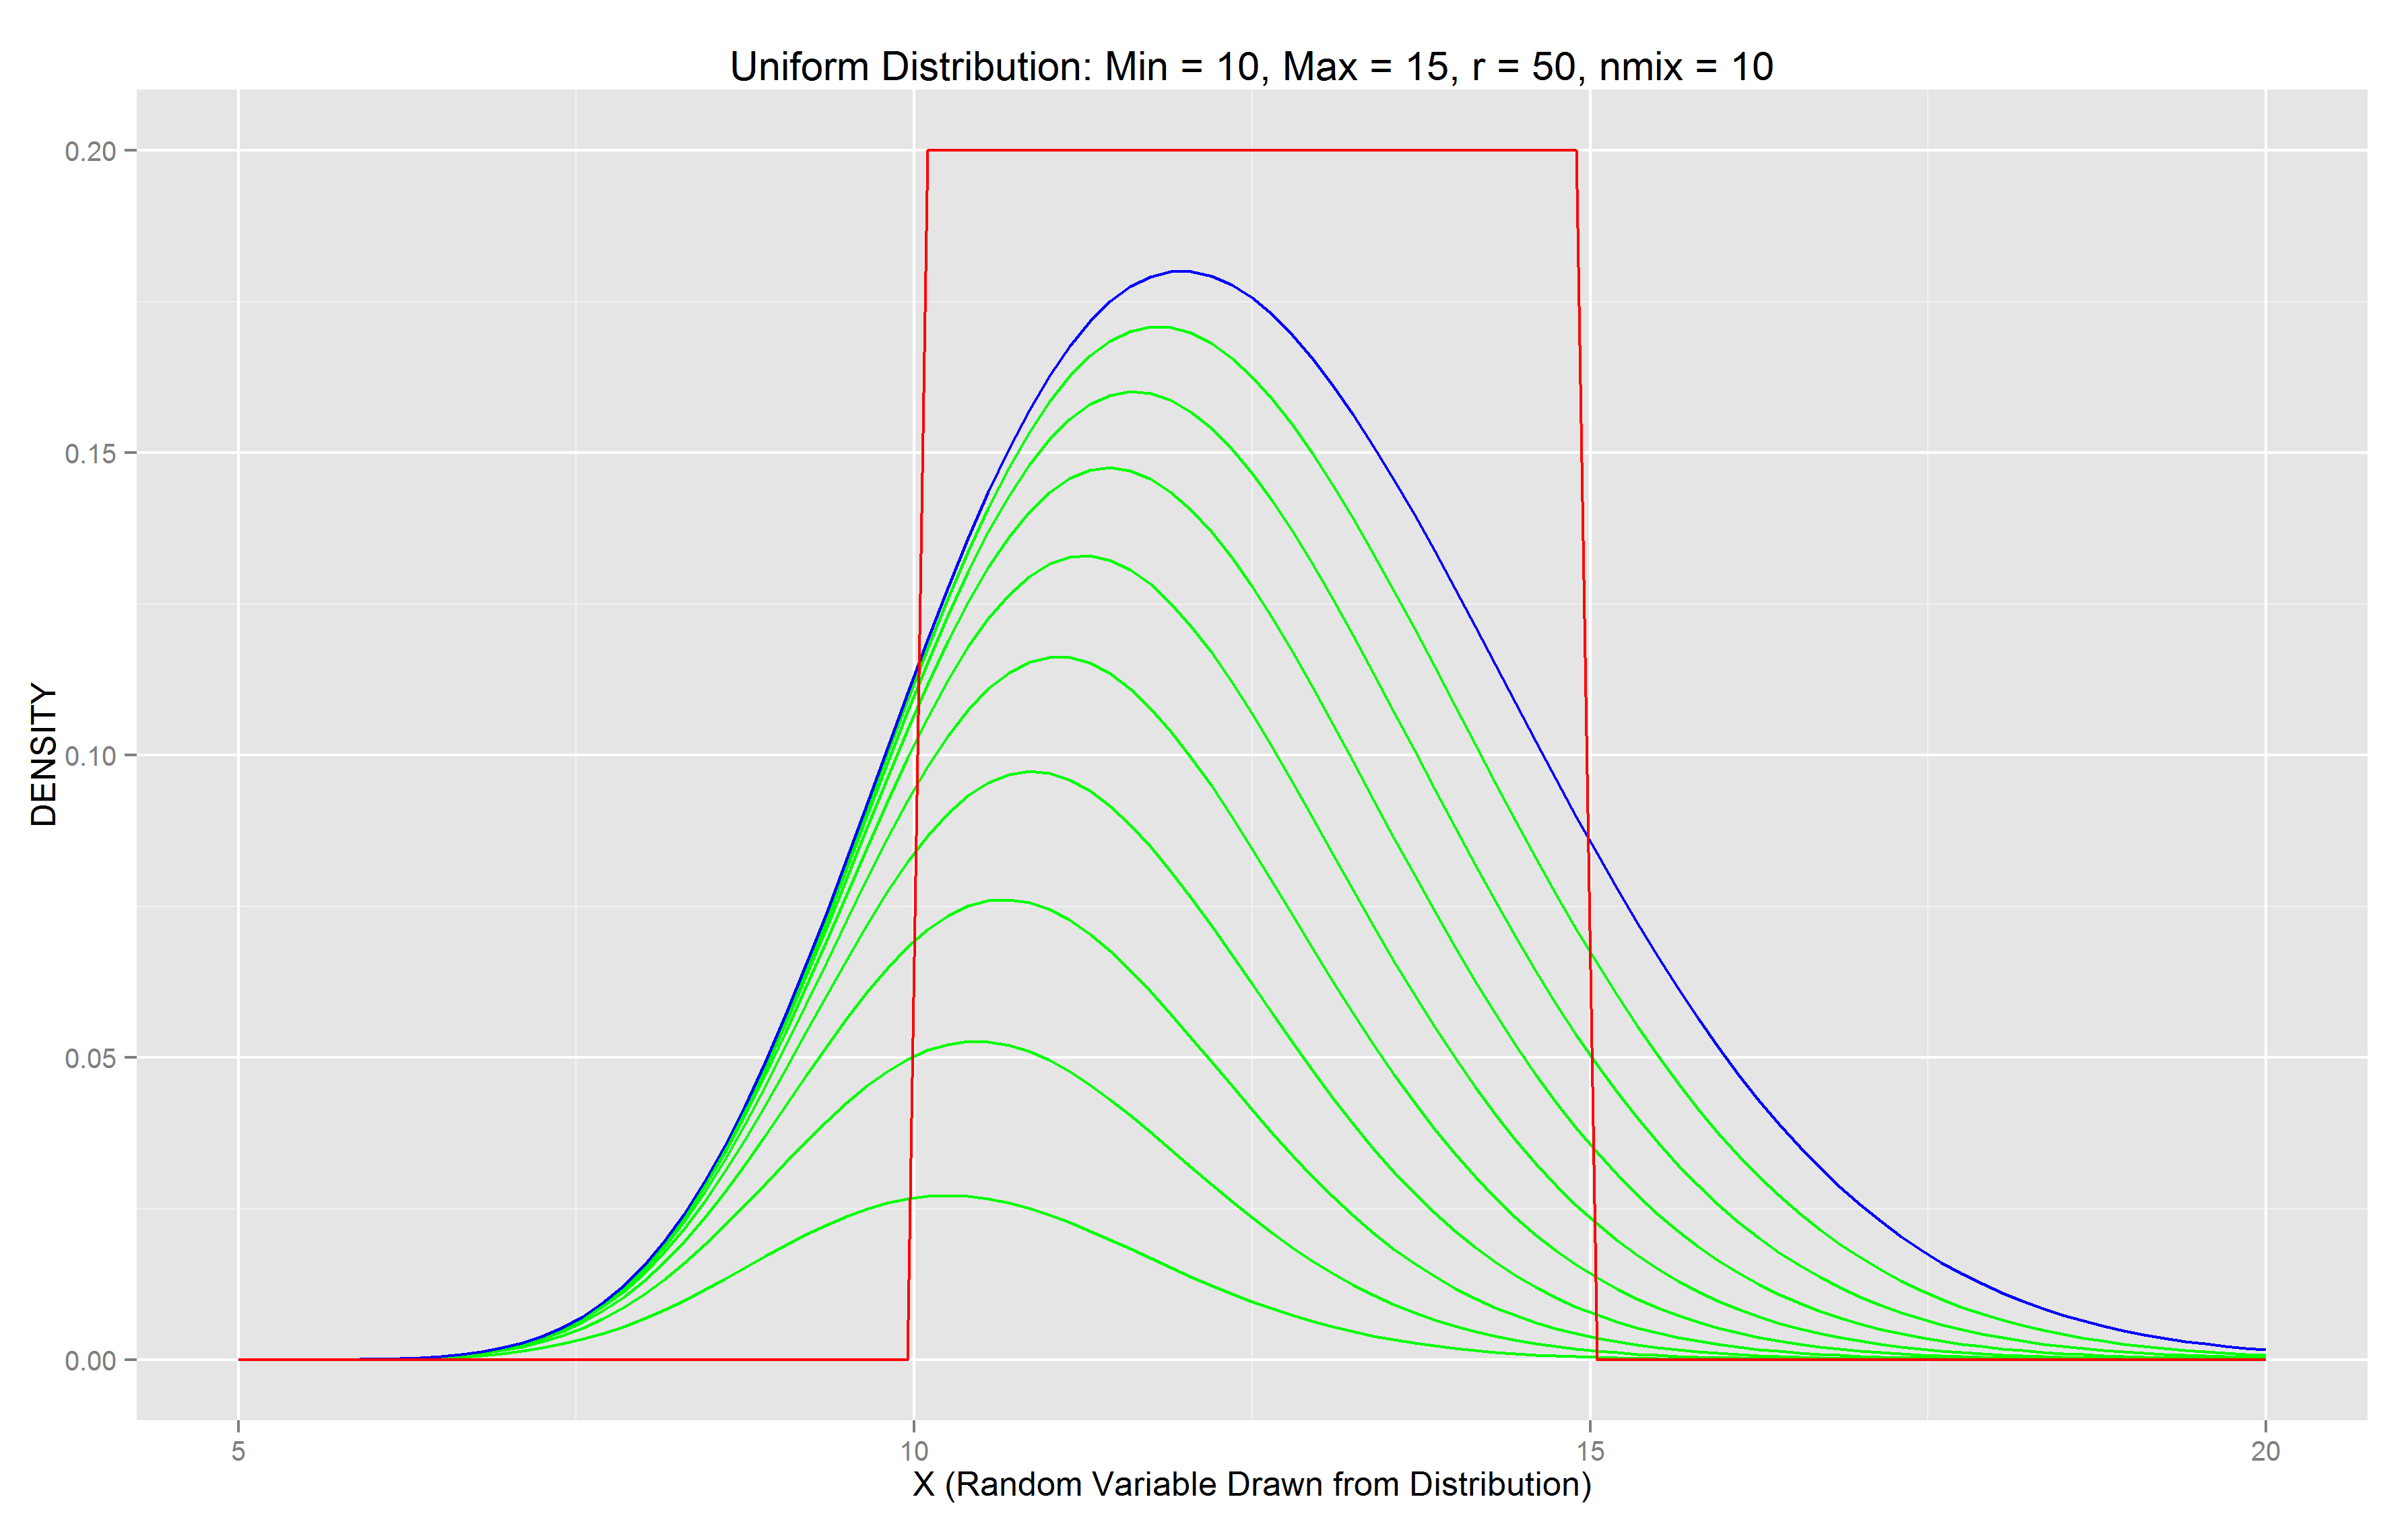
\includegraphics[scale=.27]{unifdist_10_15_50_10.png}
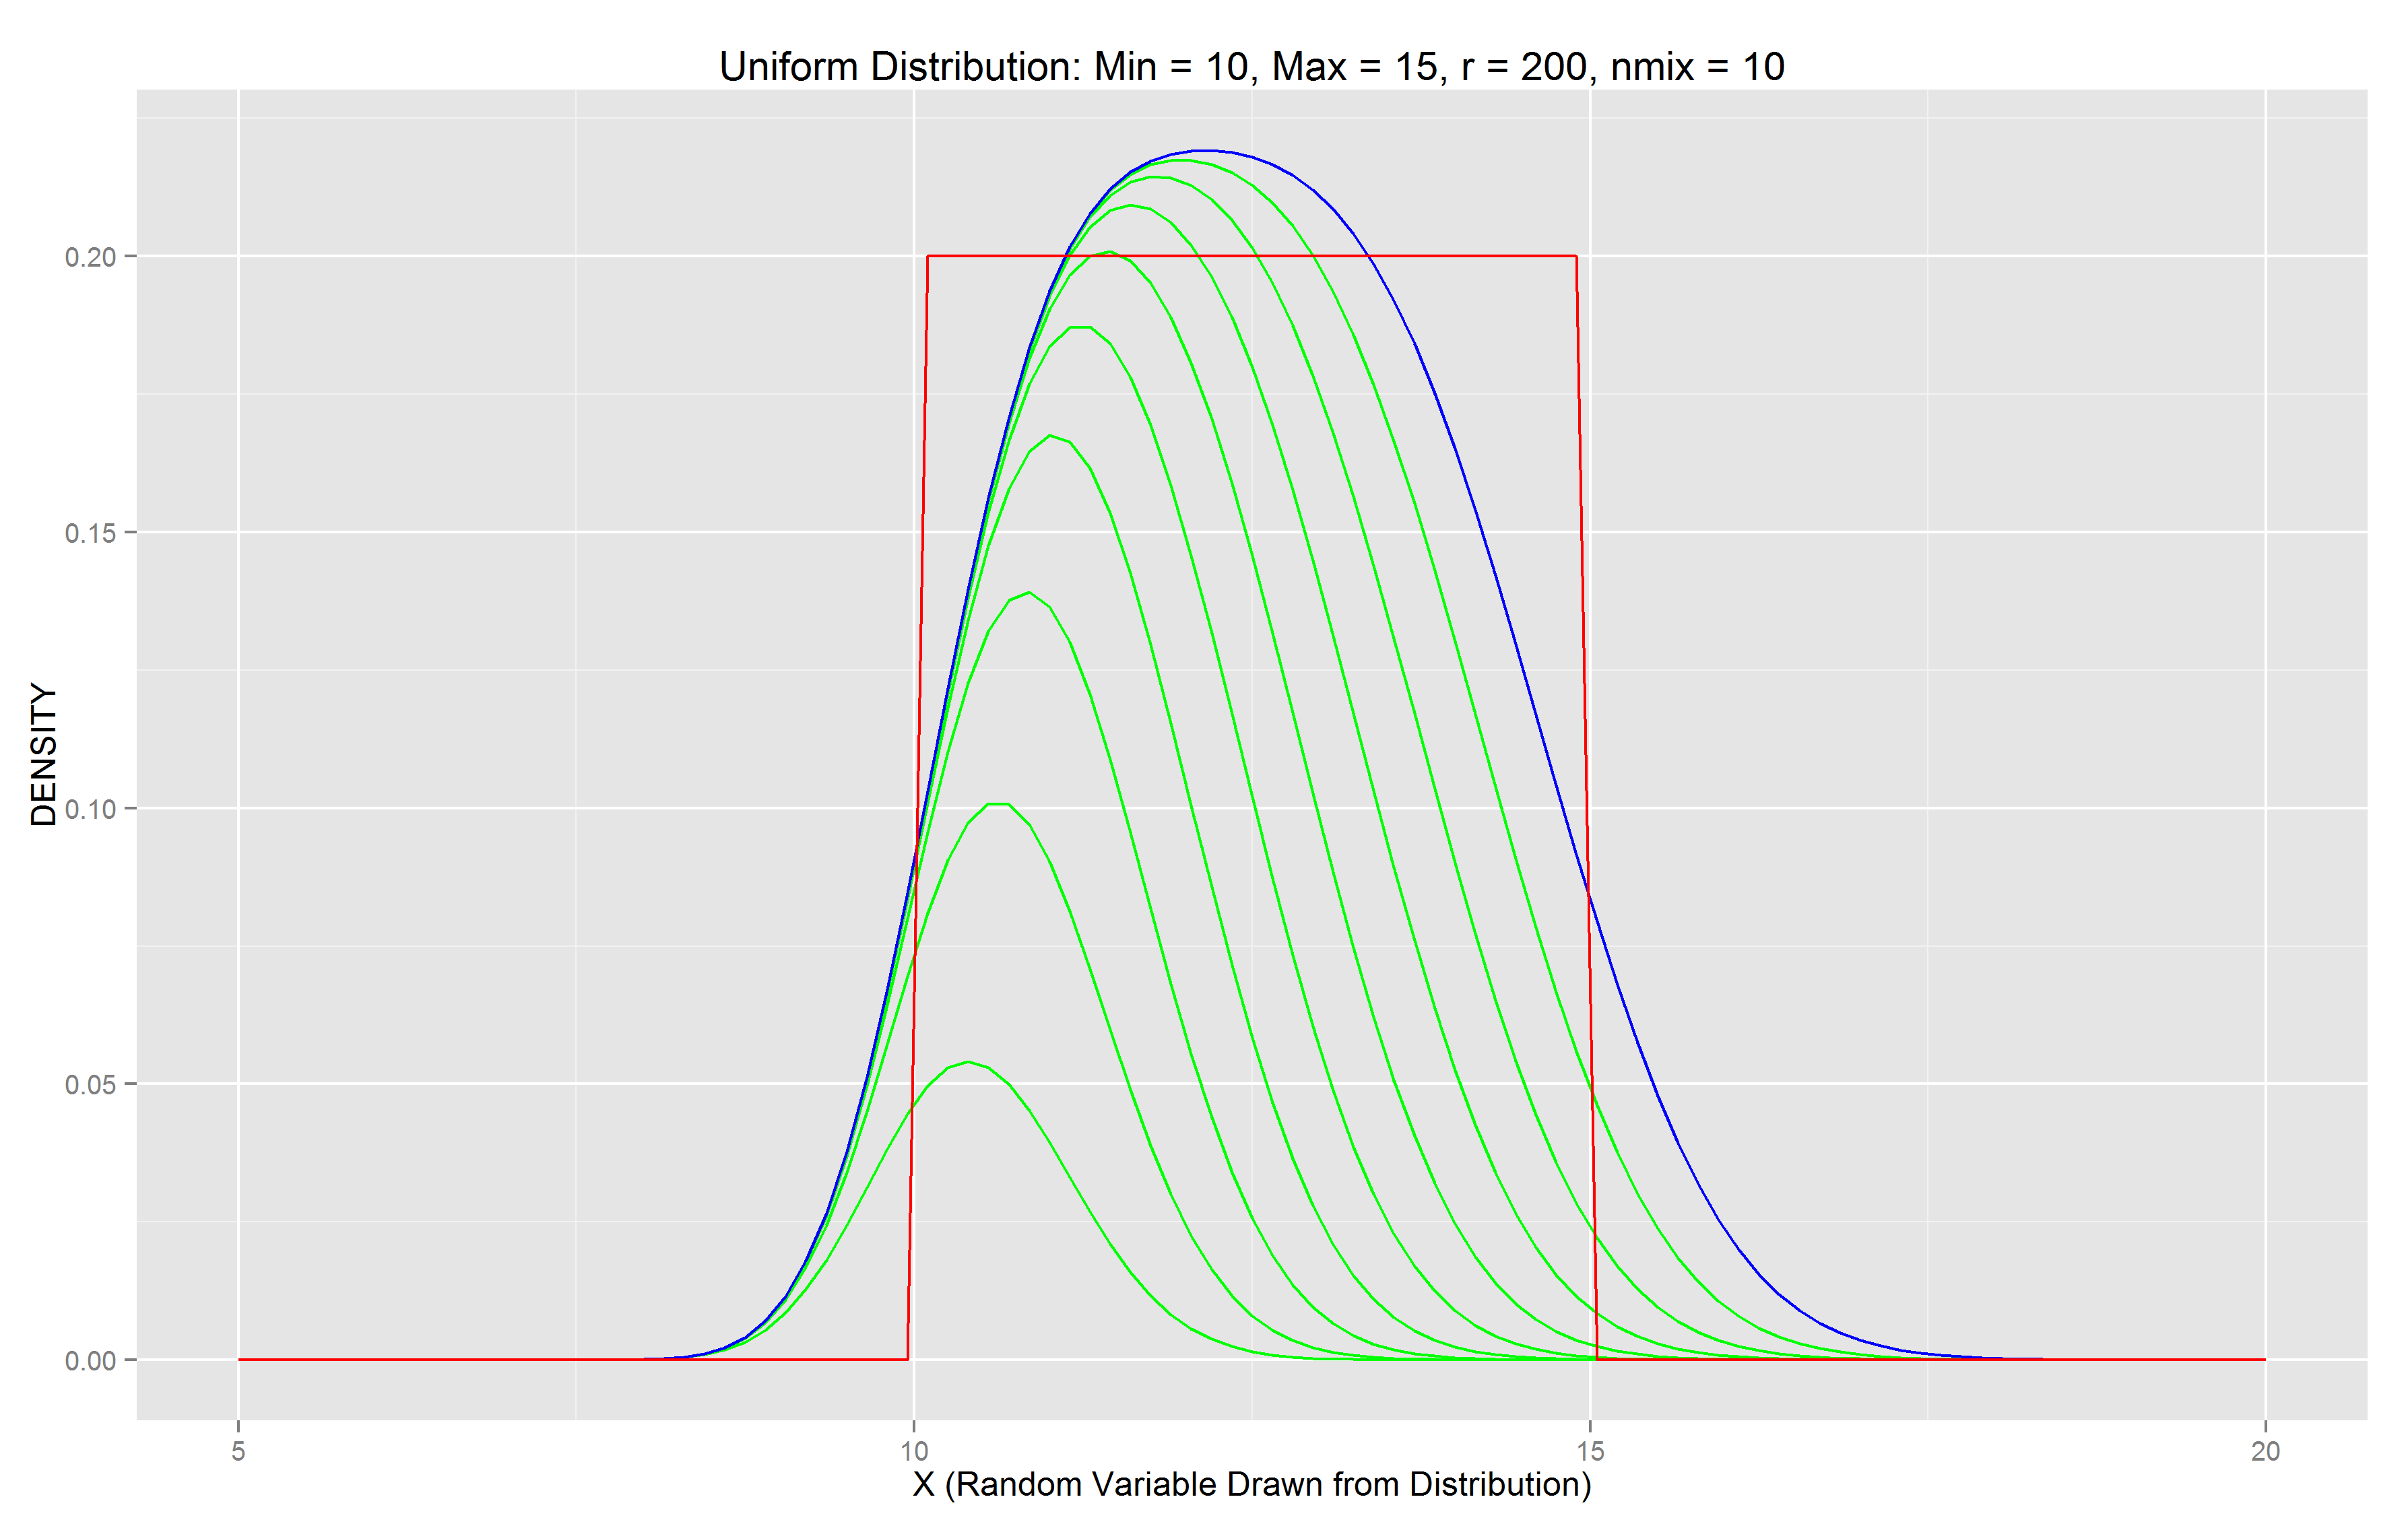
\includegraphics[scale=.27]{unifdist_10_15_200_10.png}\\
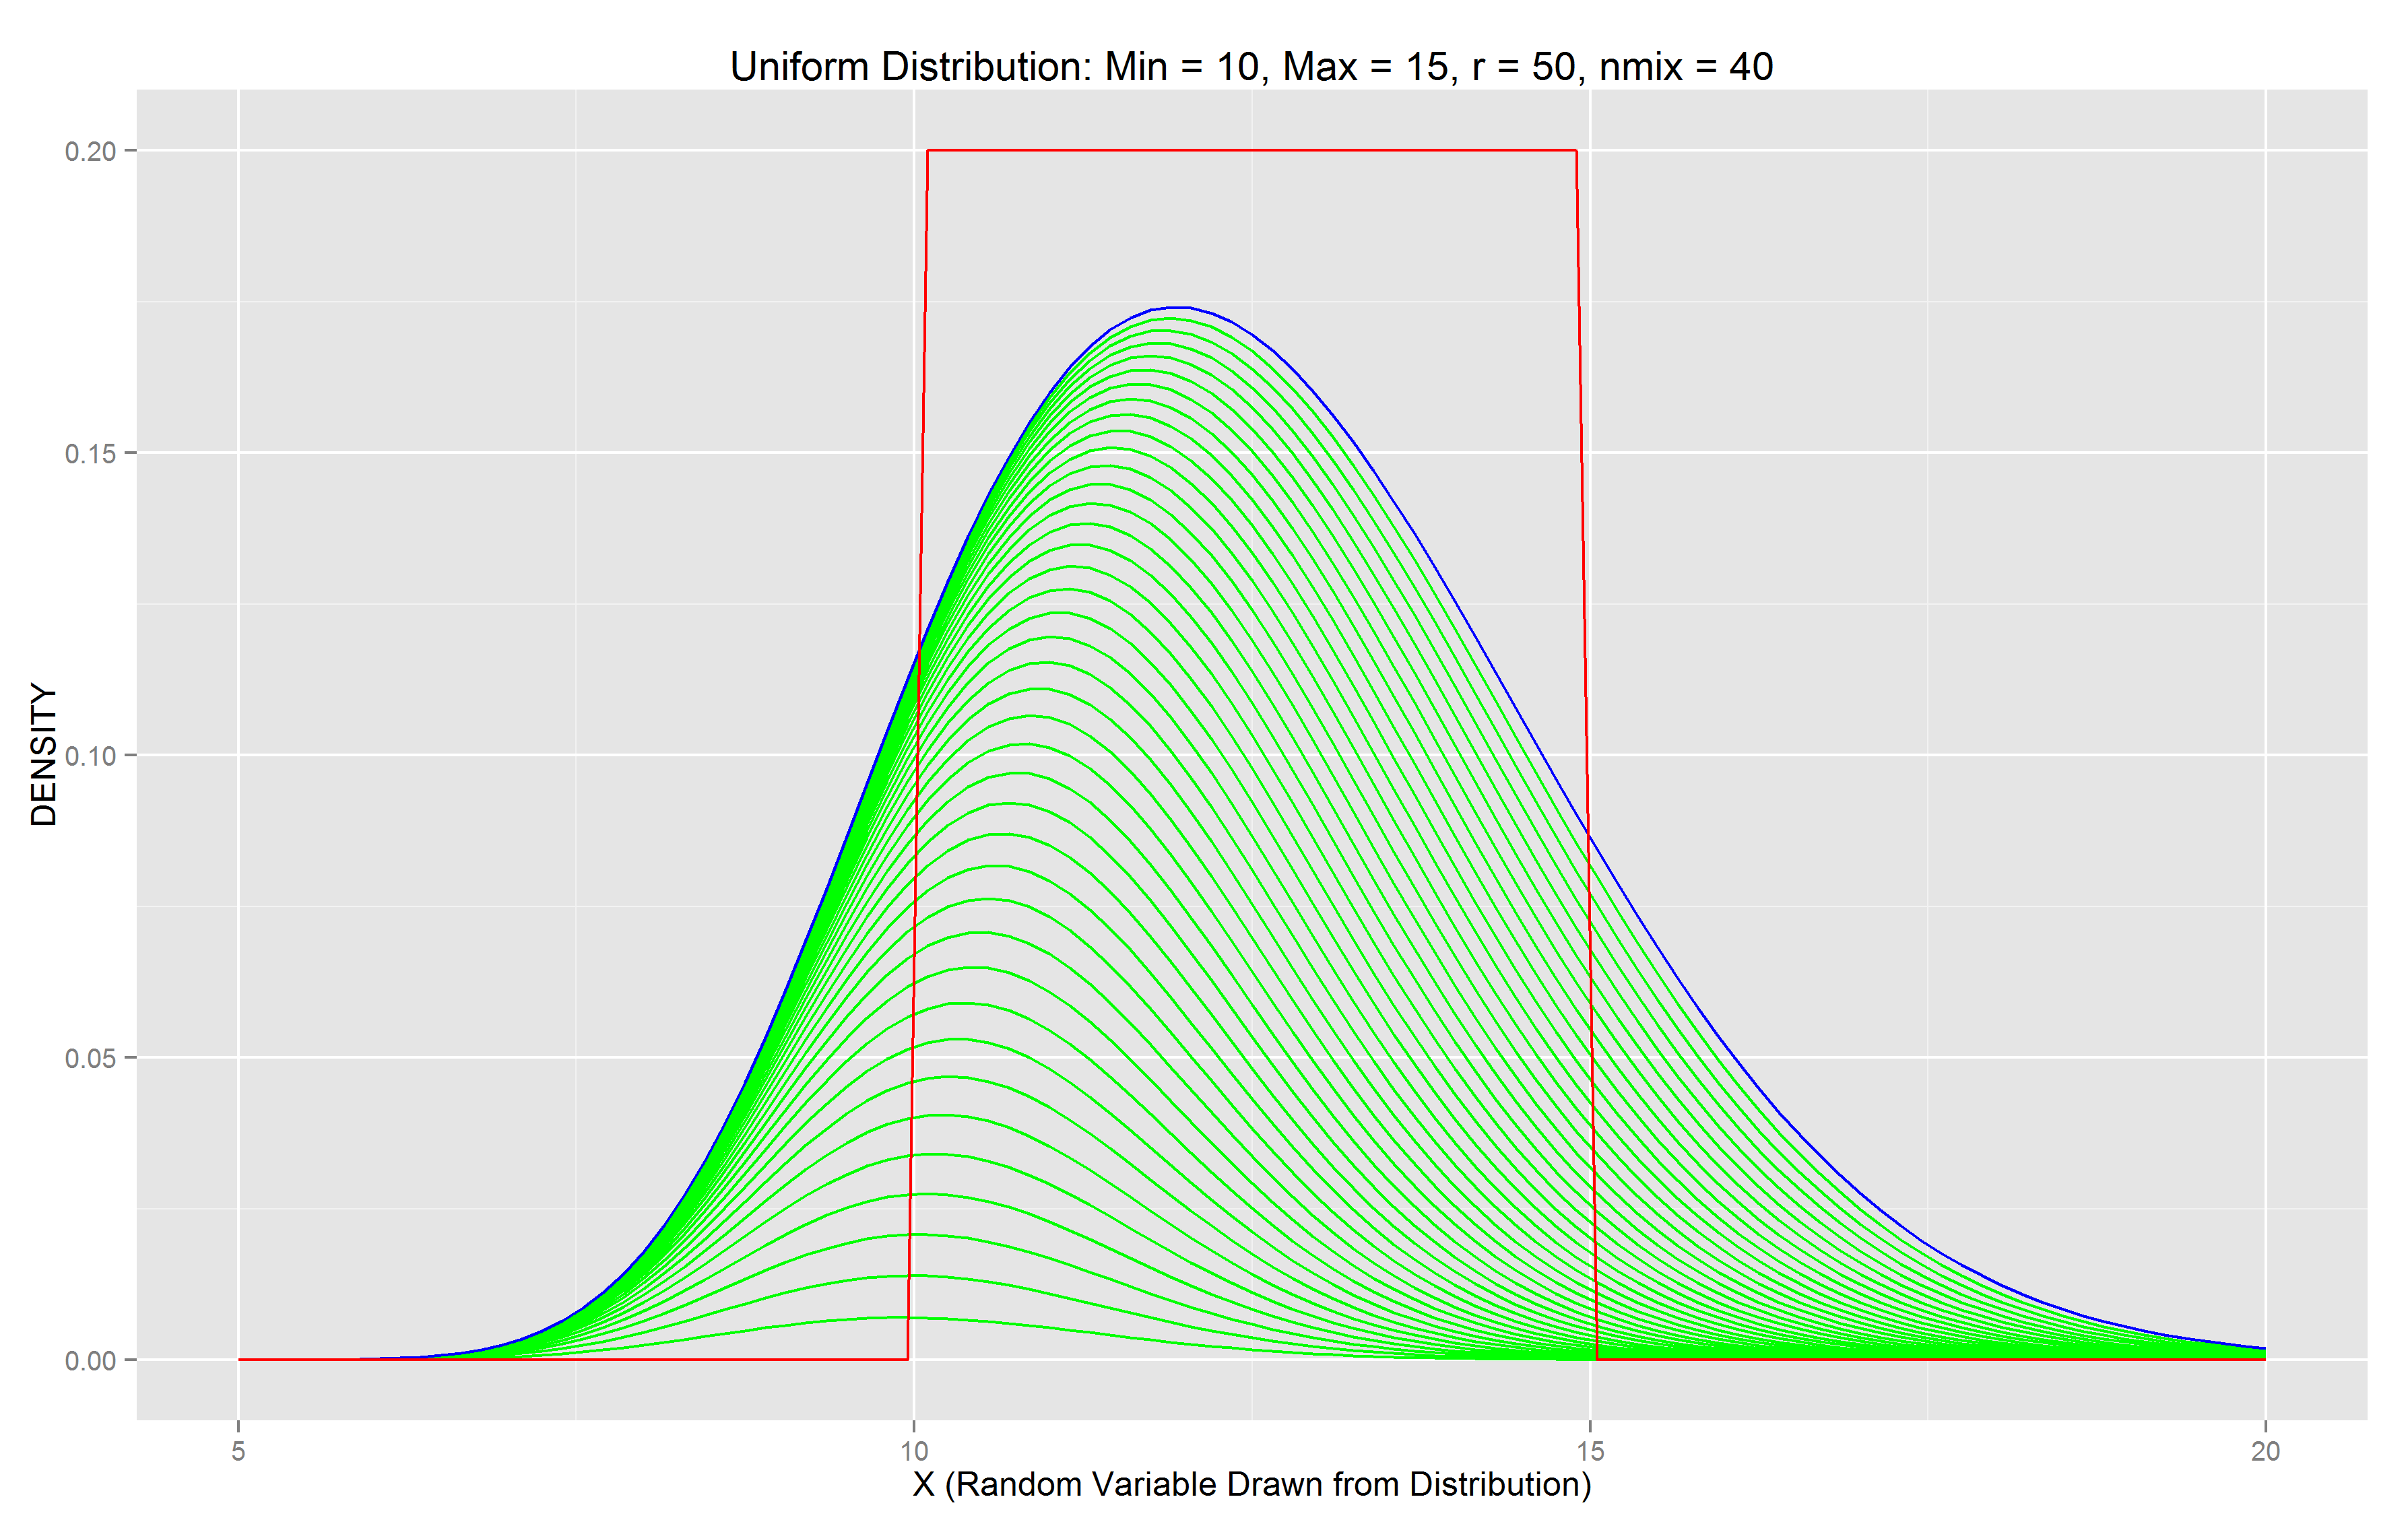
\includegraphics[scale=.27]{unifdist_10_15_50_40.png}
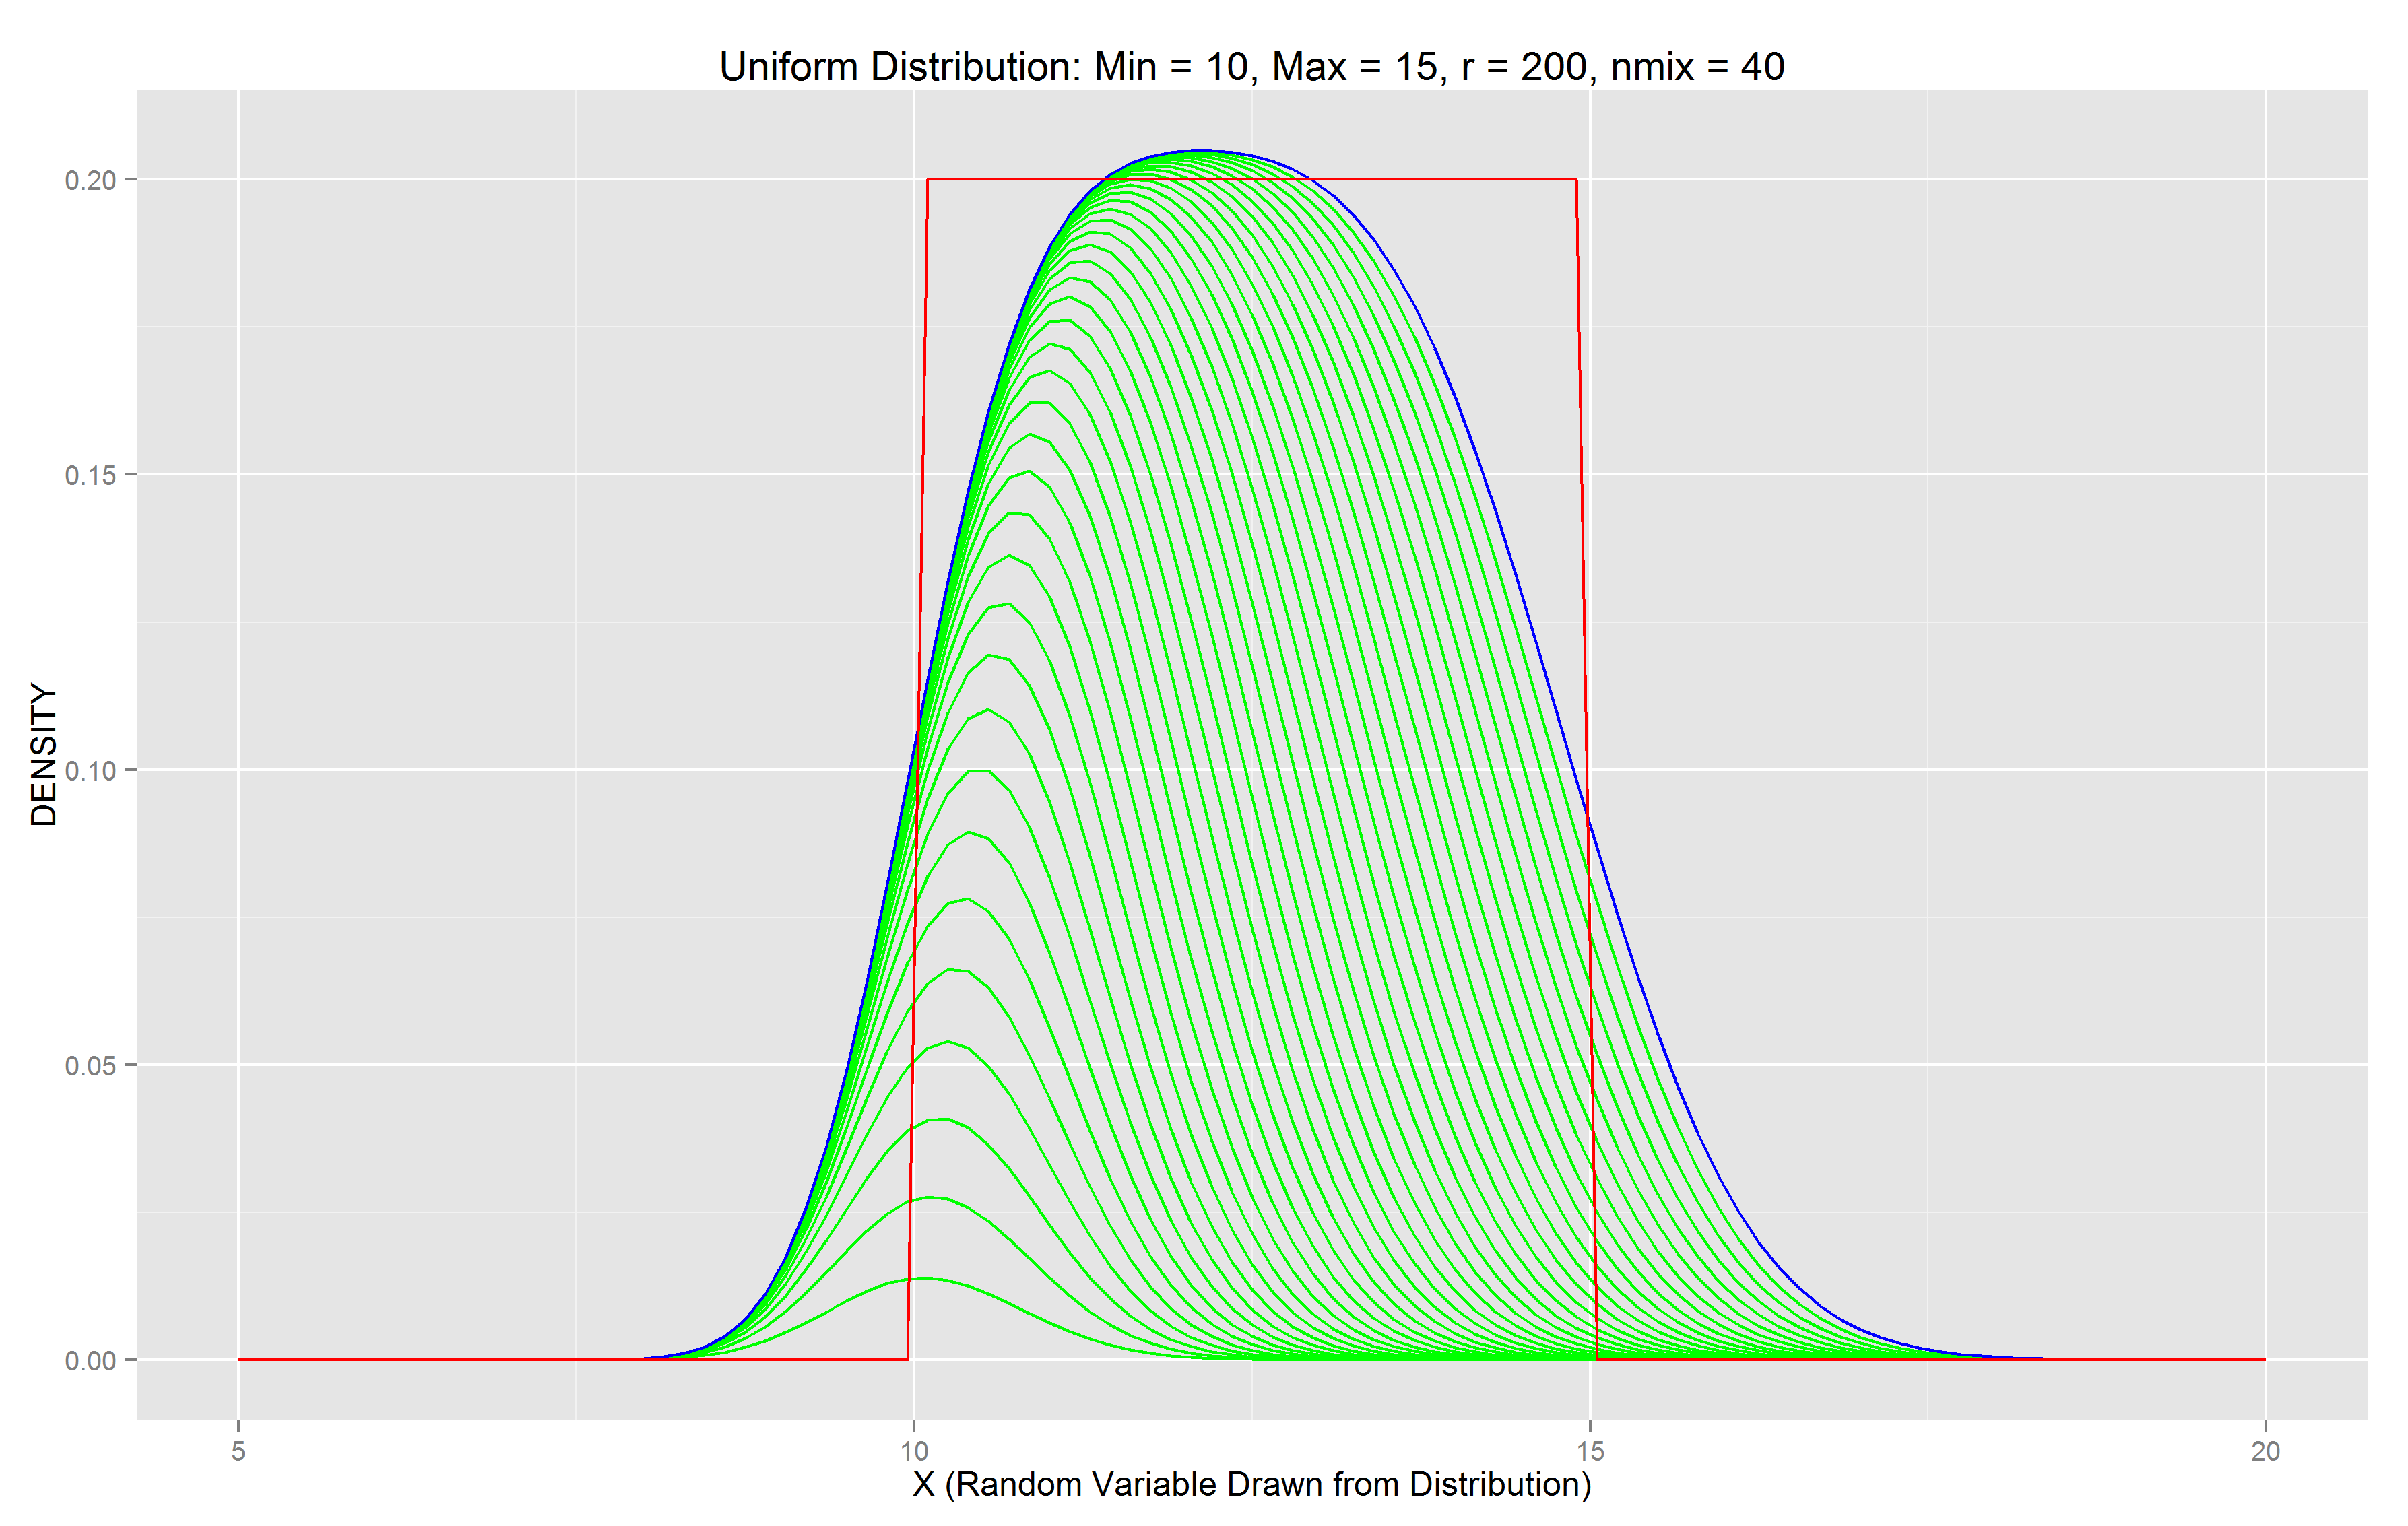
\includegraphics[scale=.27]{unifdist_10_15_200_40.png}\\
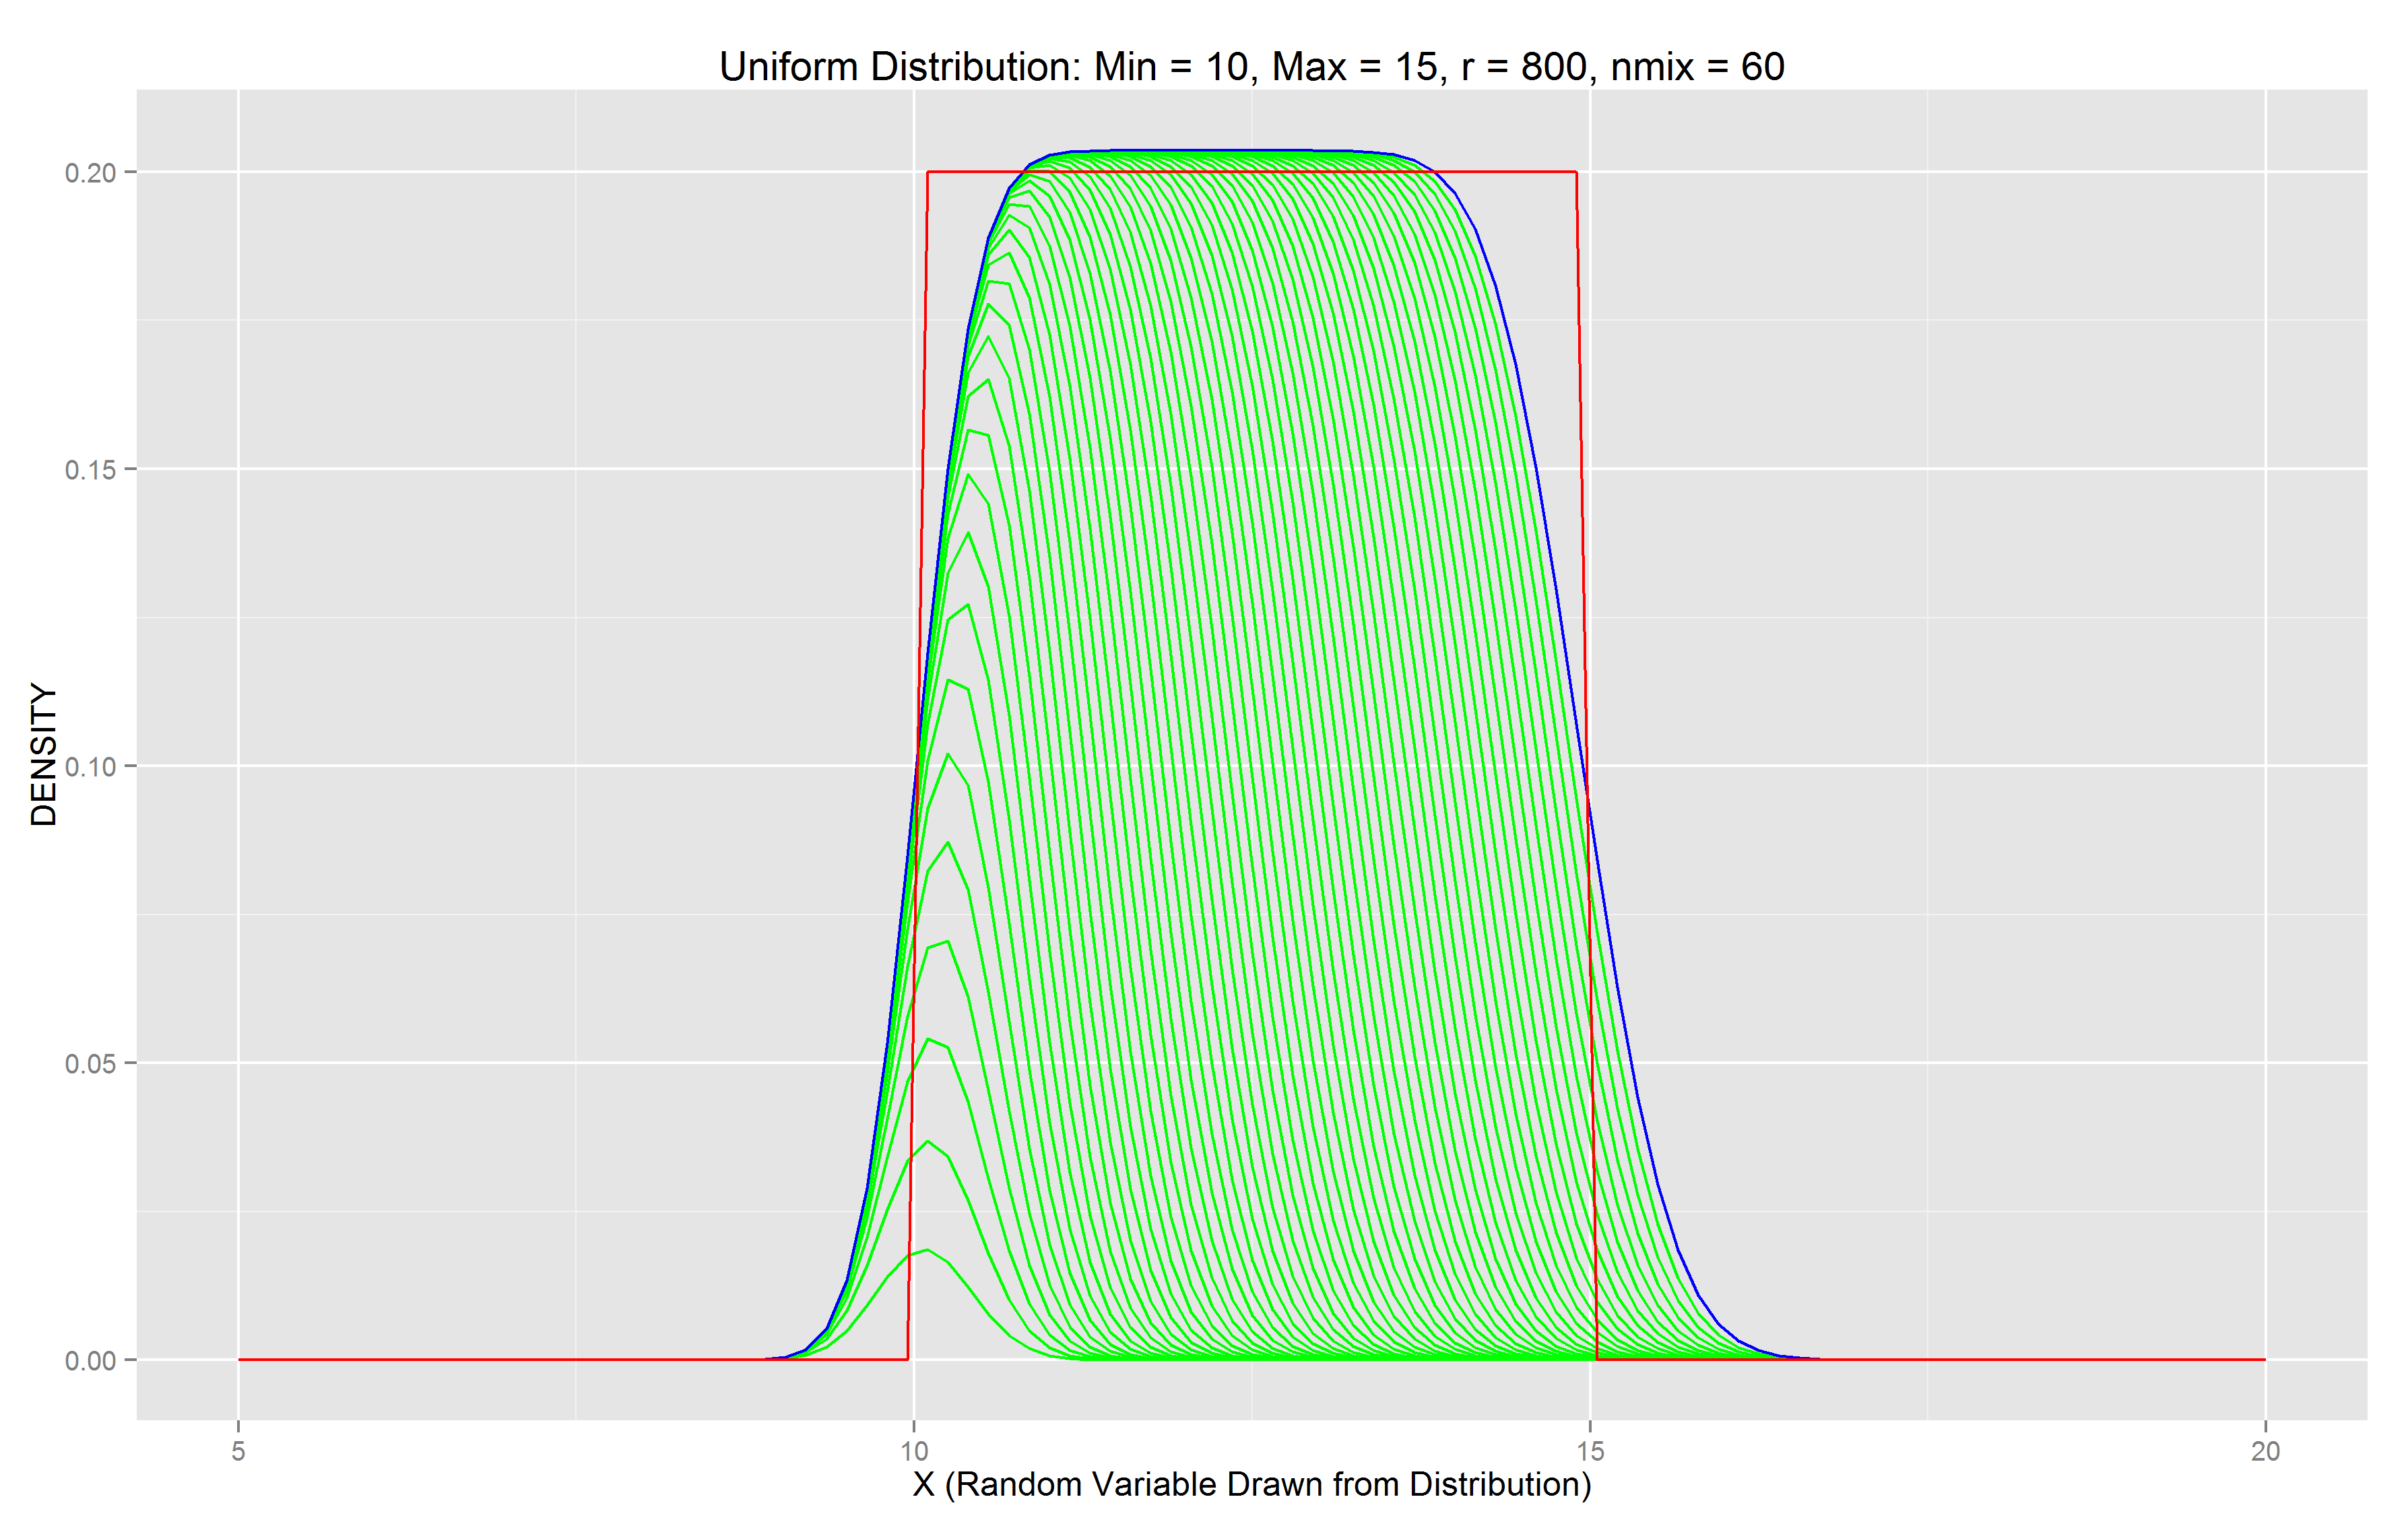
\includegraphics[scale=.54]{unifdist_10_15_800_60.png}
\end{figure}


\begin{figure}[H]
\centering
\newpage
\Large{For a normal distribution with mean = 10, standard deviation = 4:}\\
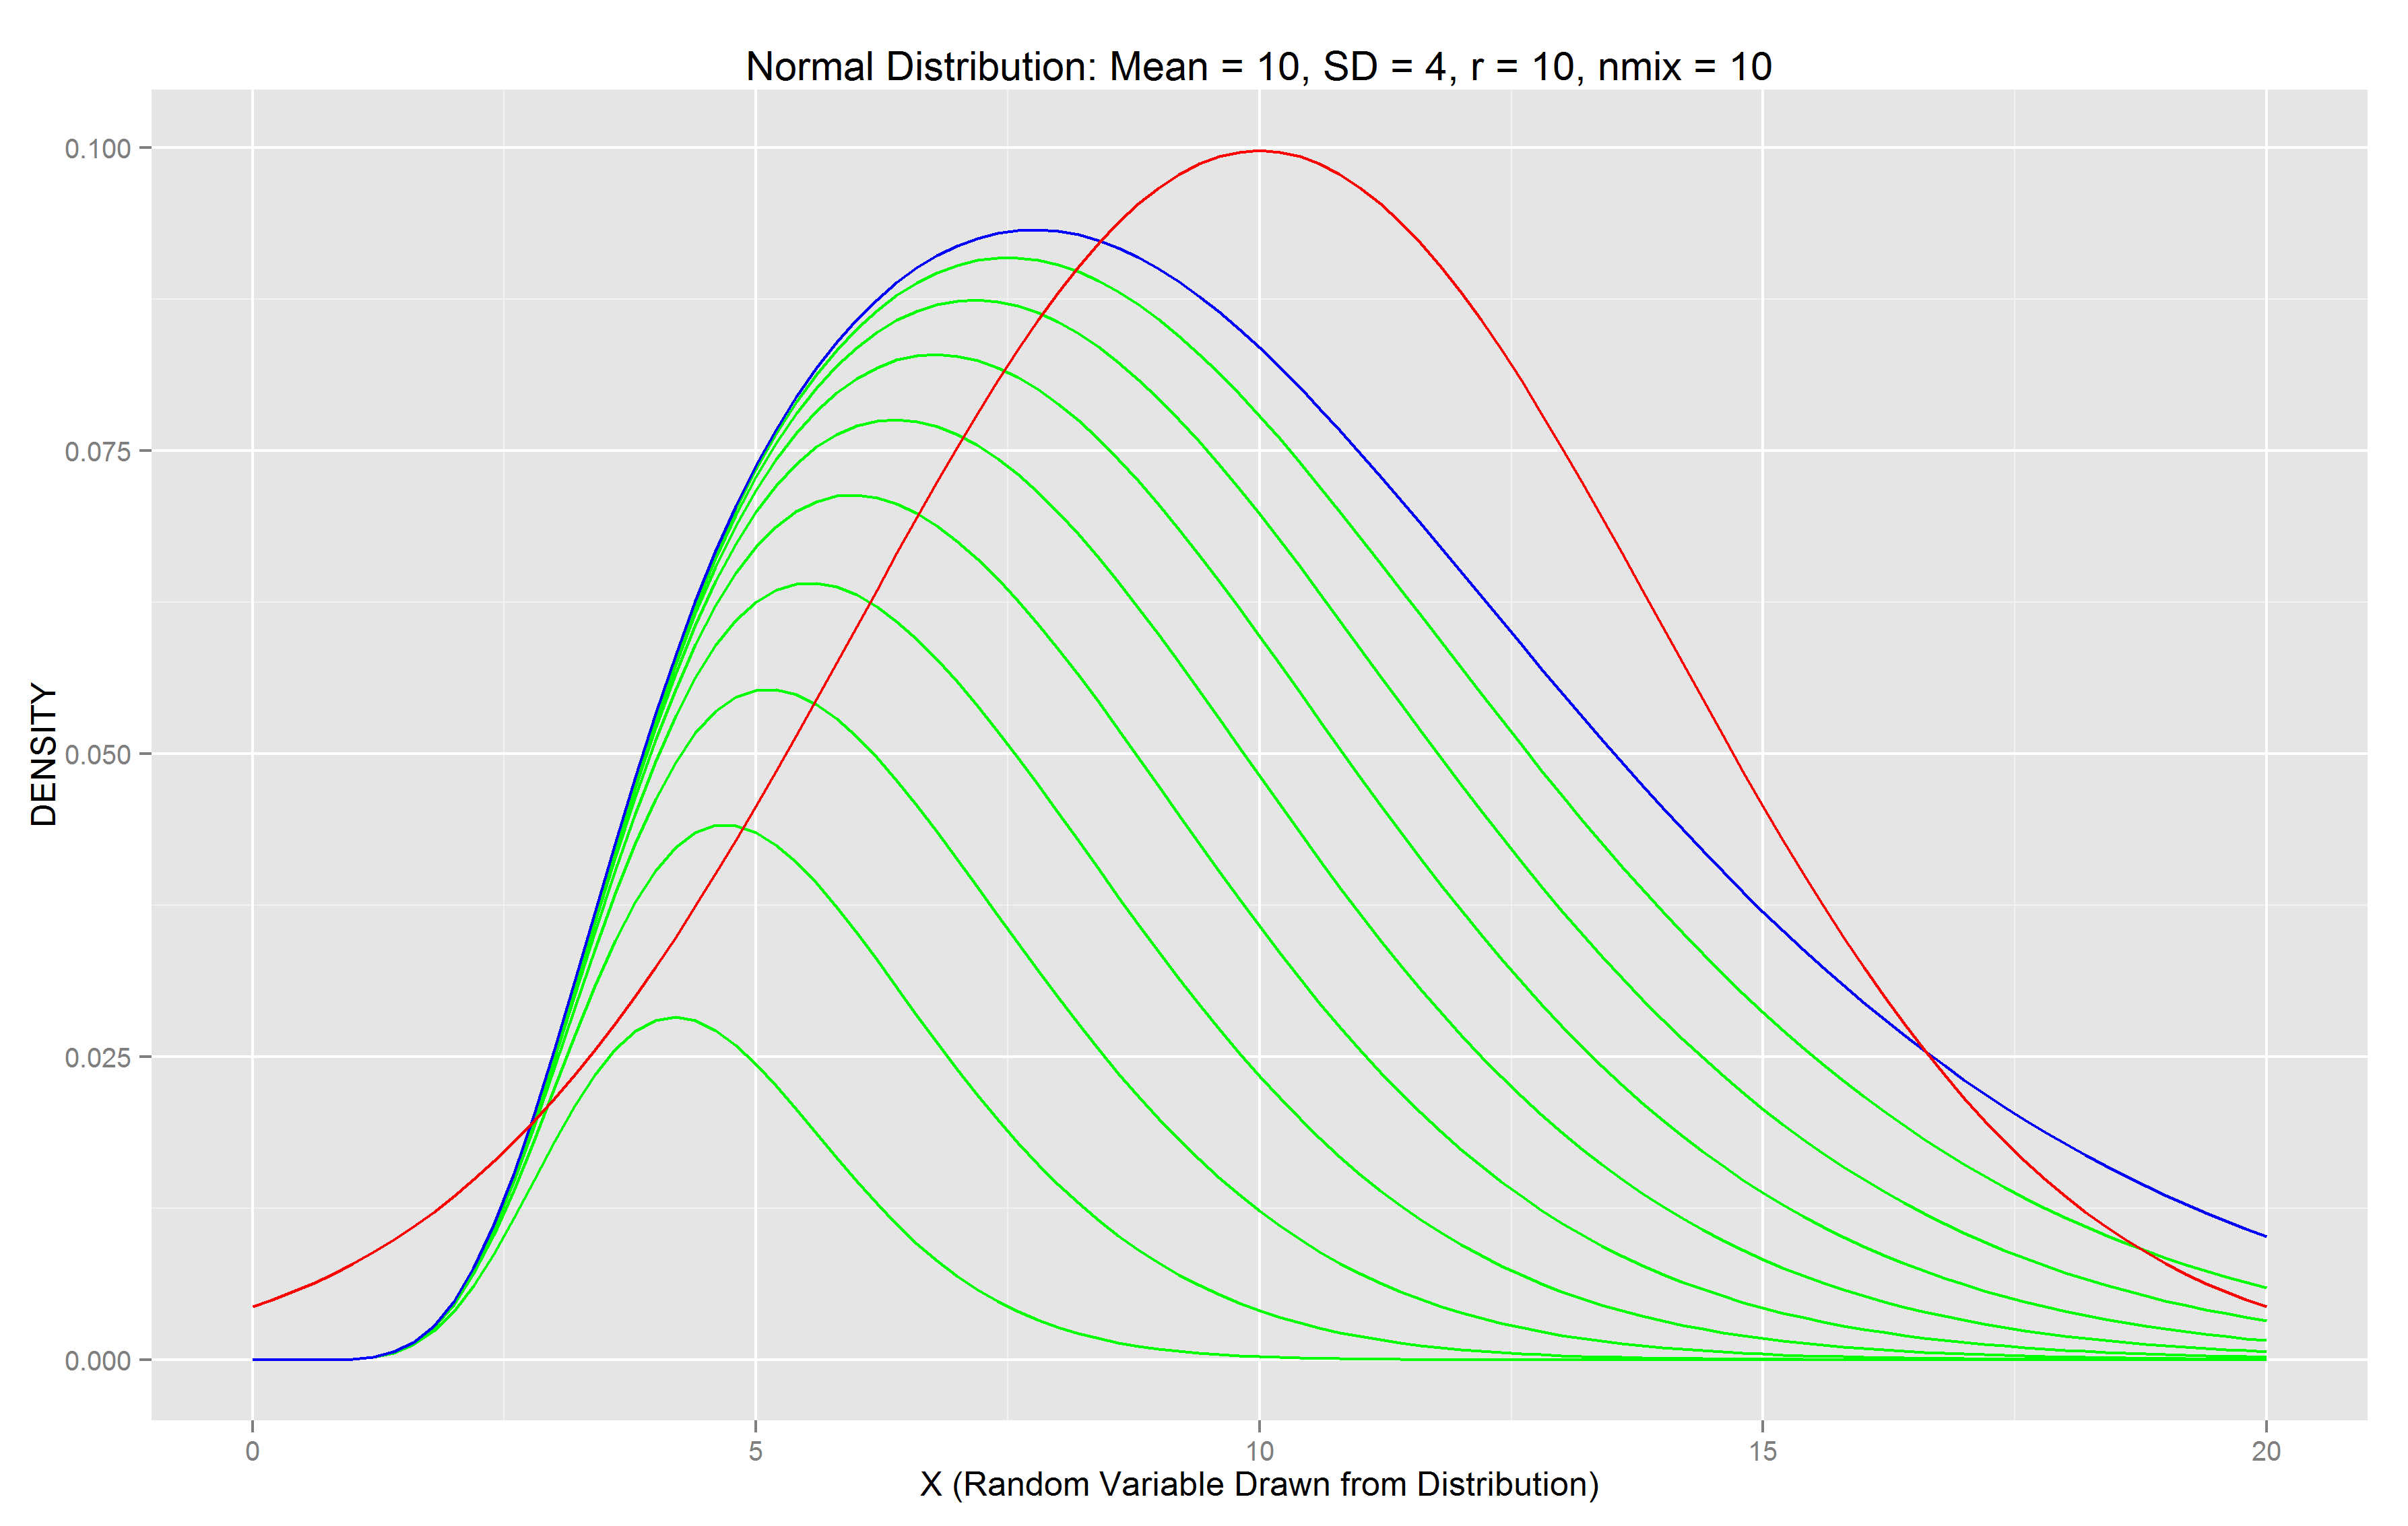
\includegraphics[scale=.27]{normdist_10_4_10_10.png}
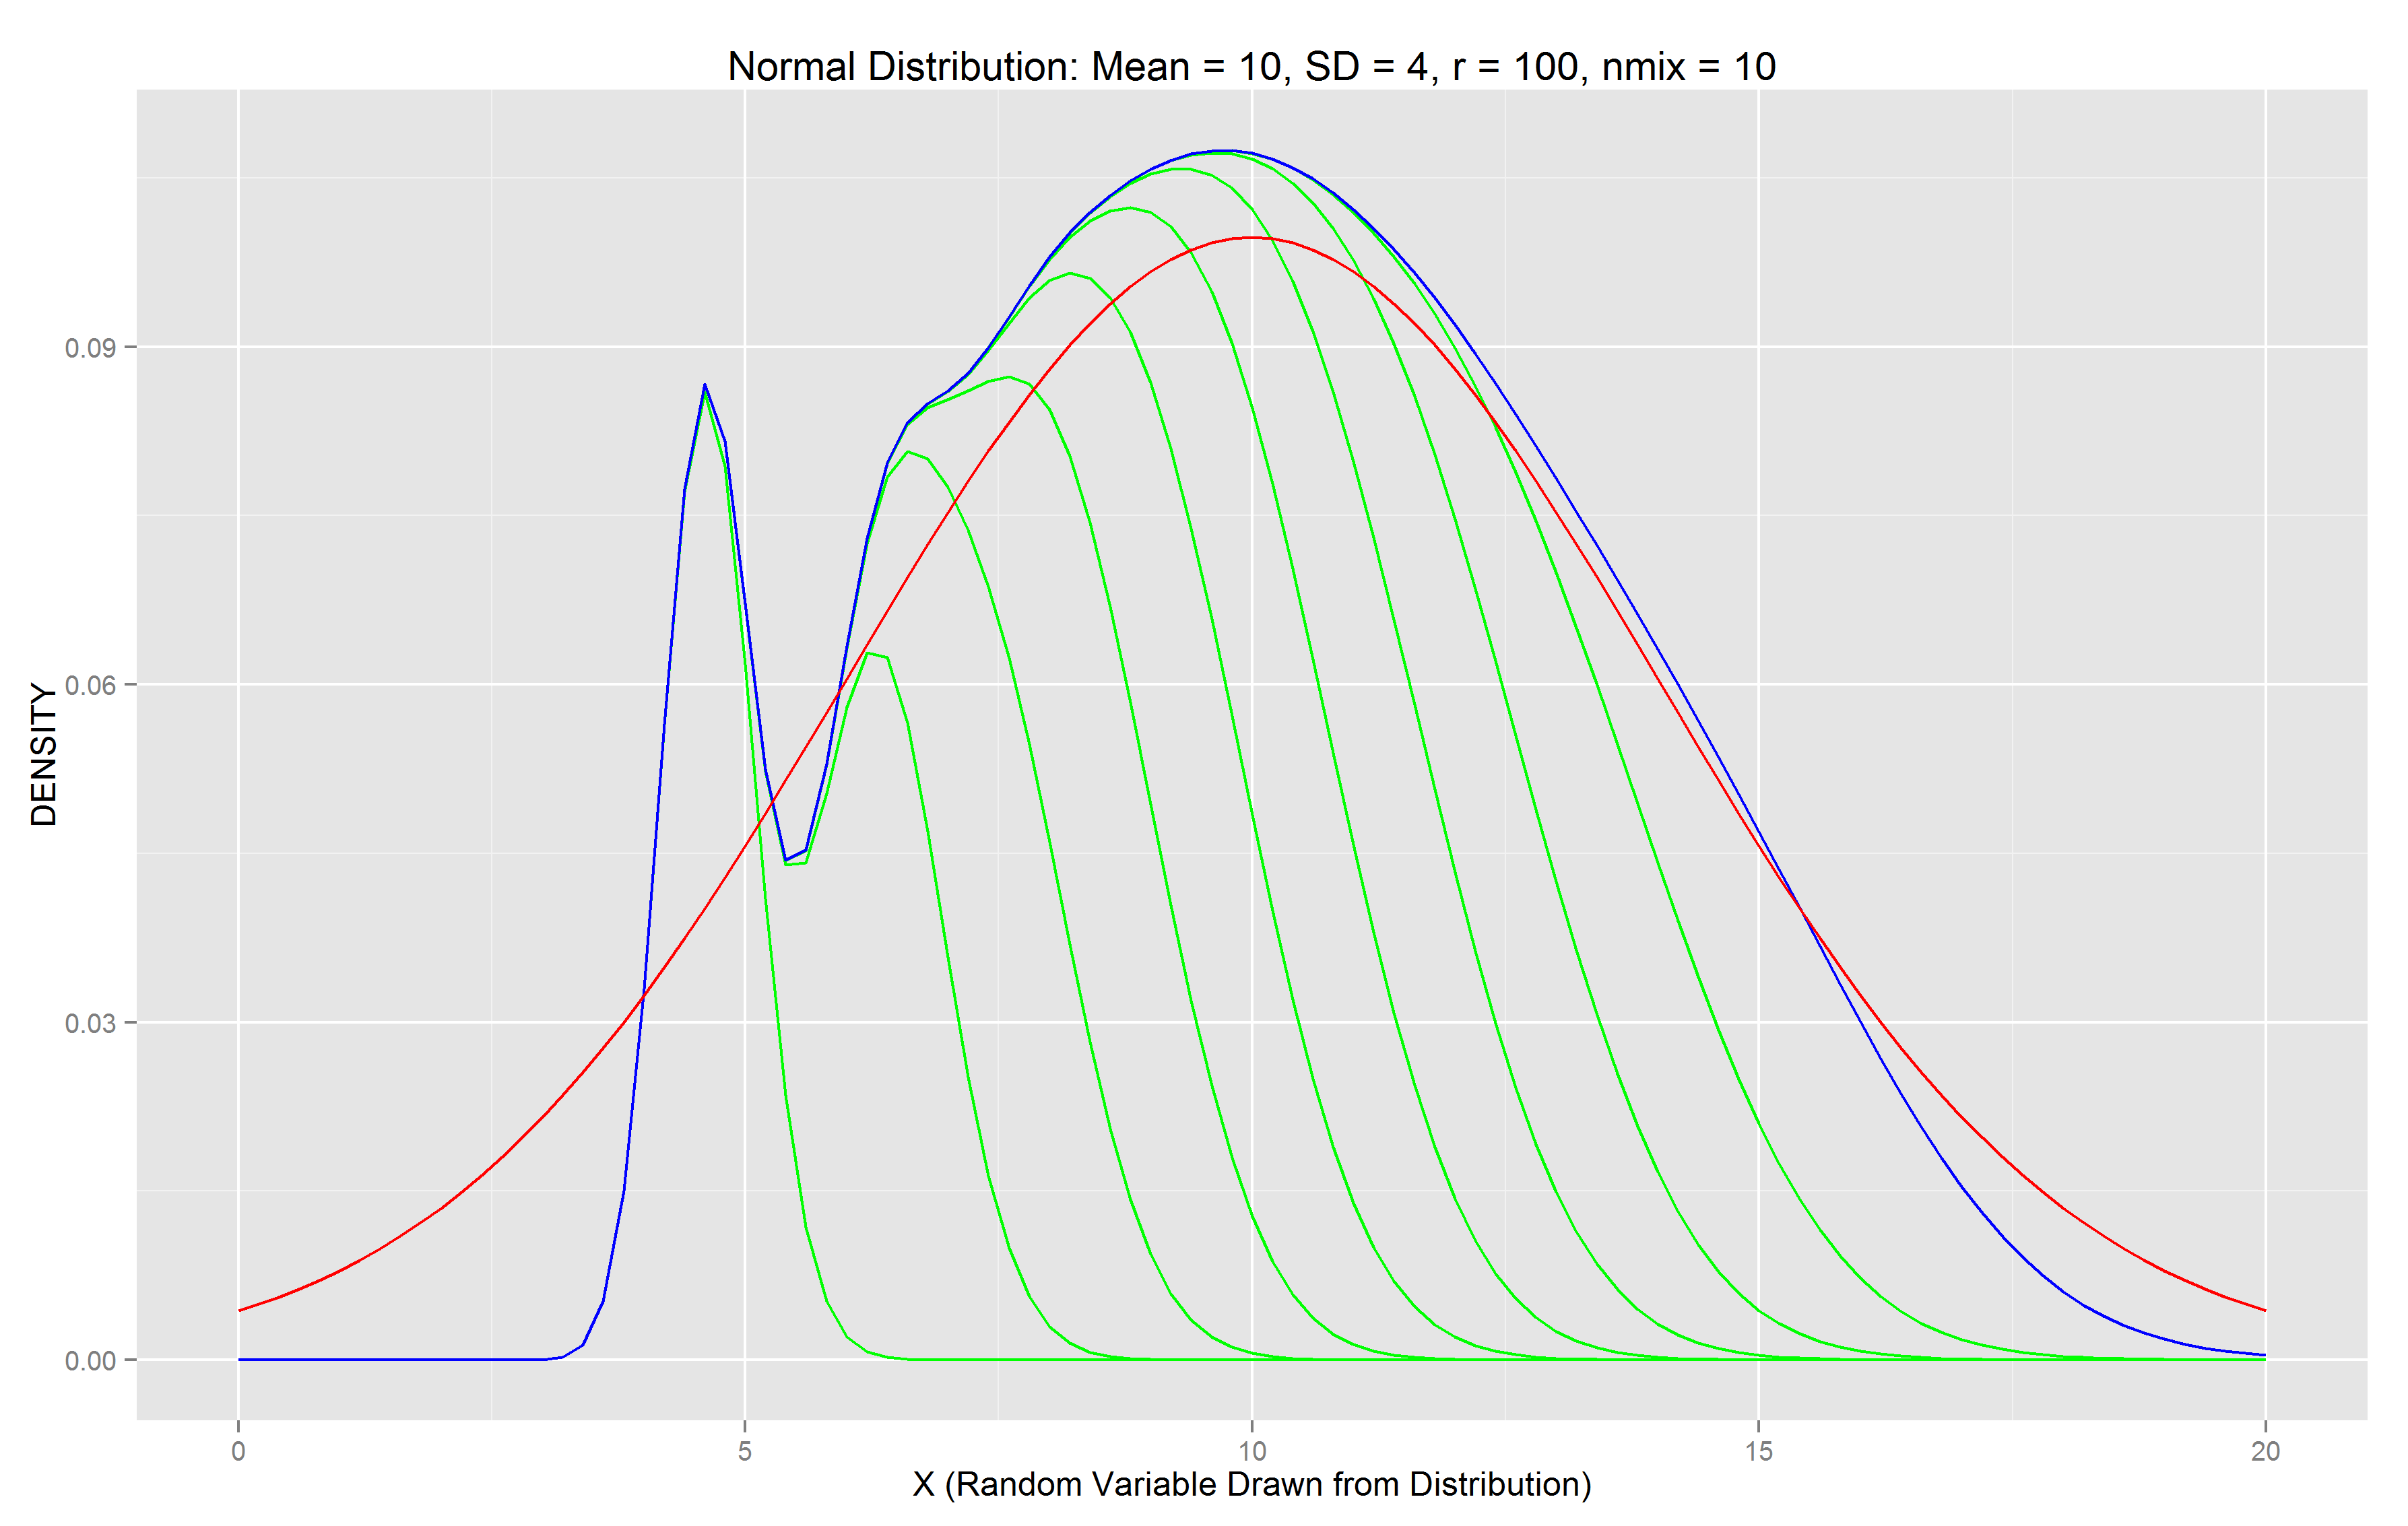
\includegraphics[scale=.27]{normdist_10_4_100_10.png}\\
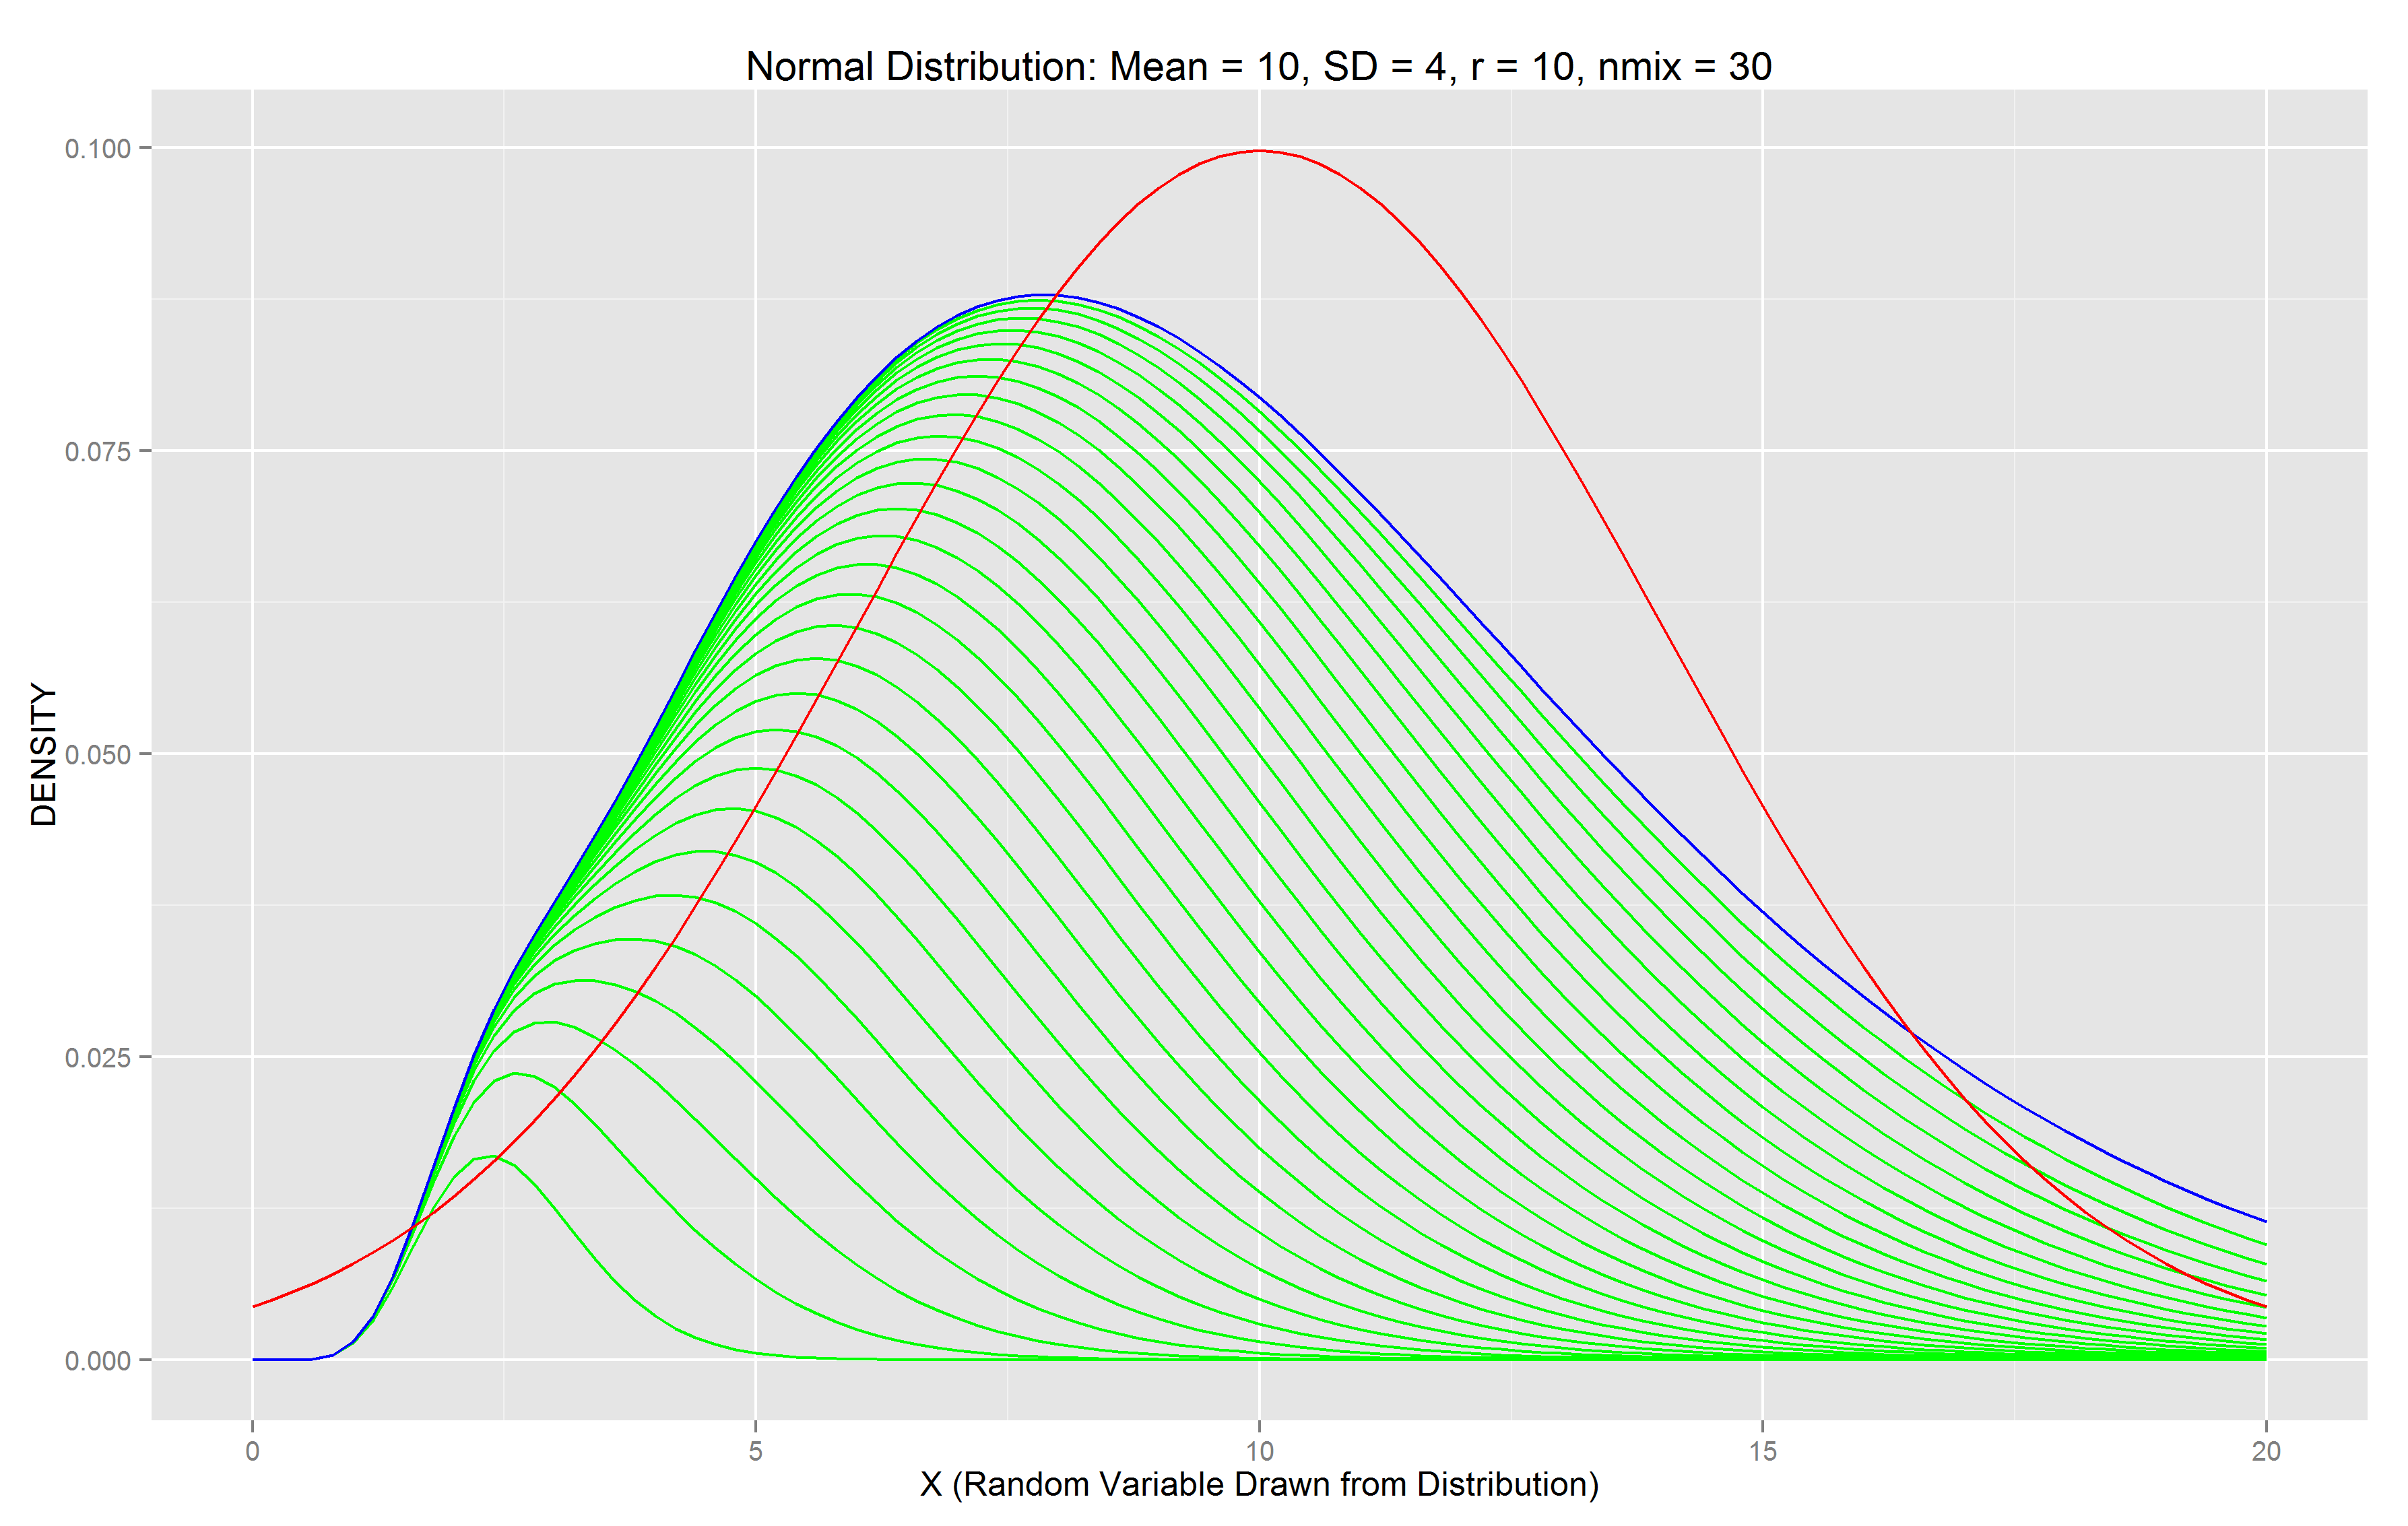
\includegraphics[scale=.27]{normdist_10_4_10_30.png}
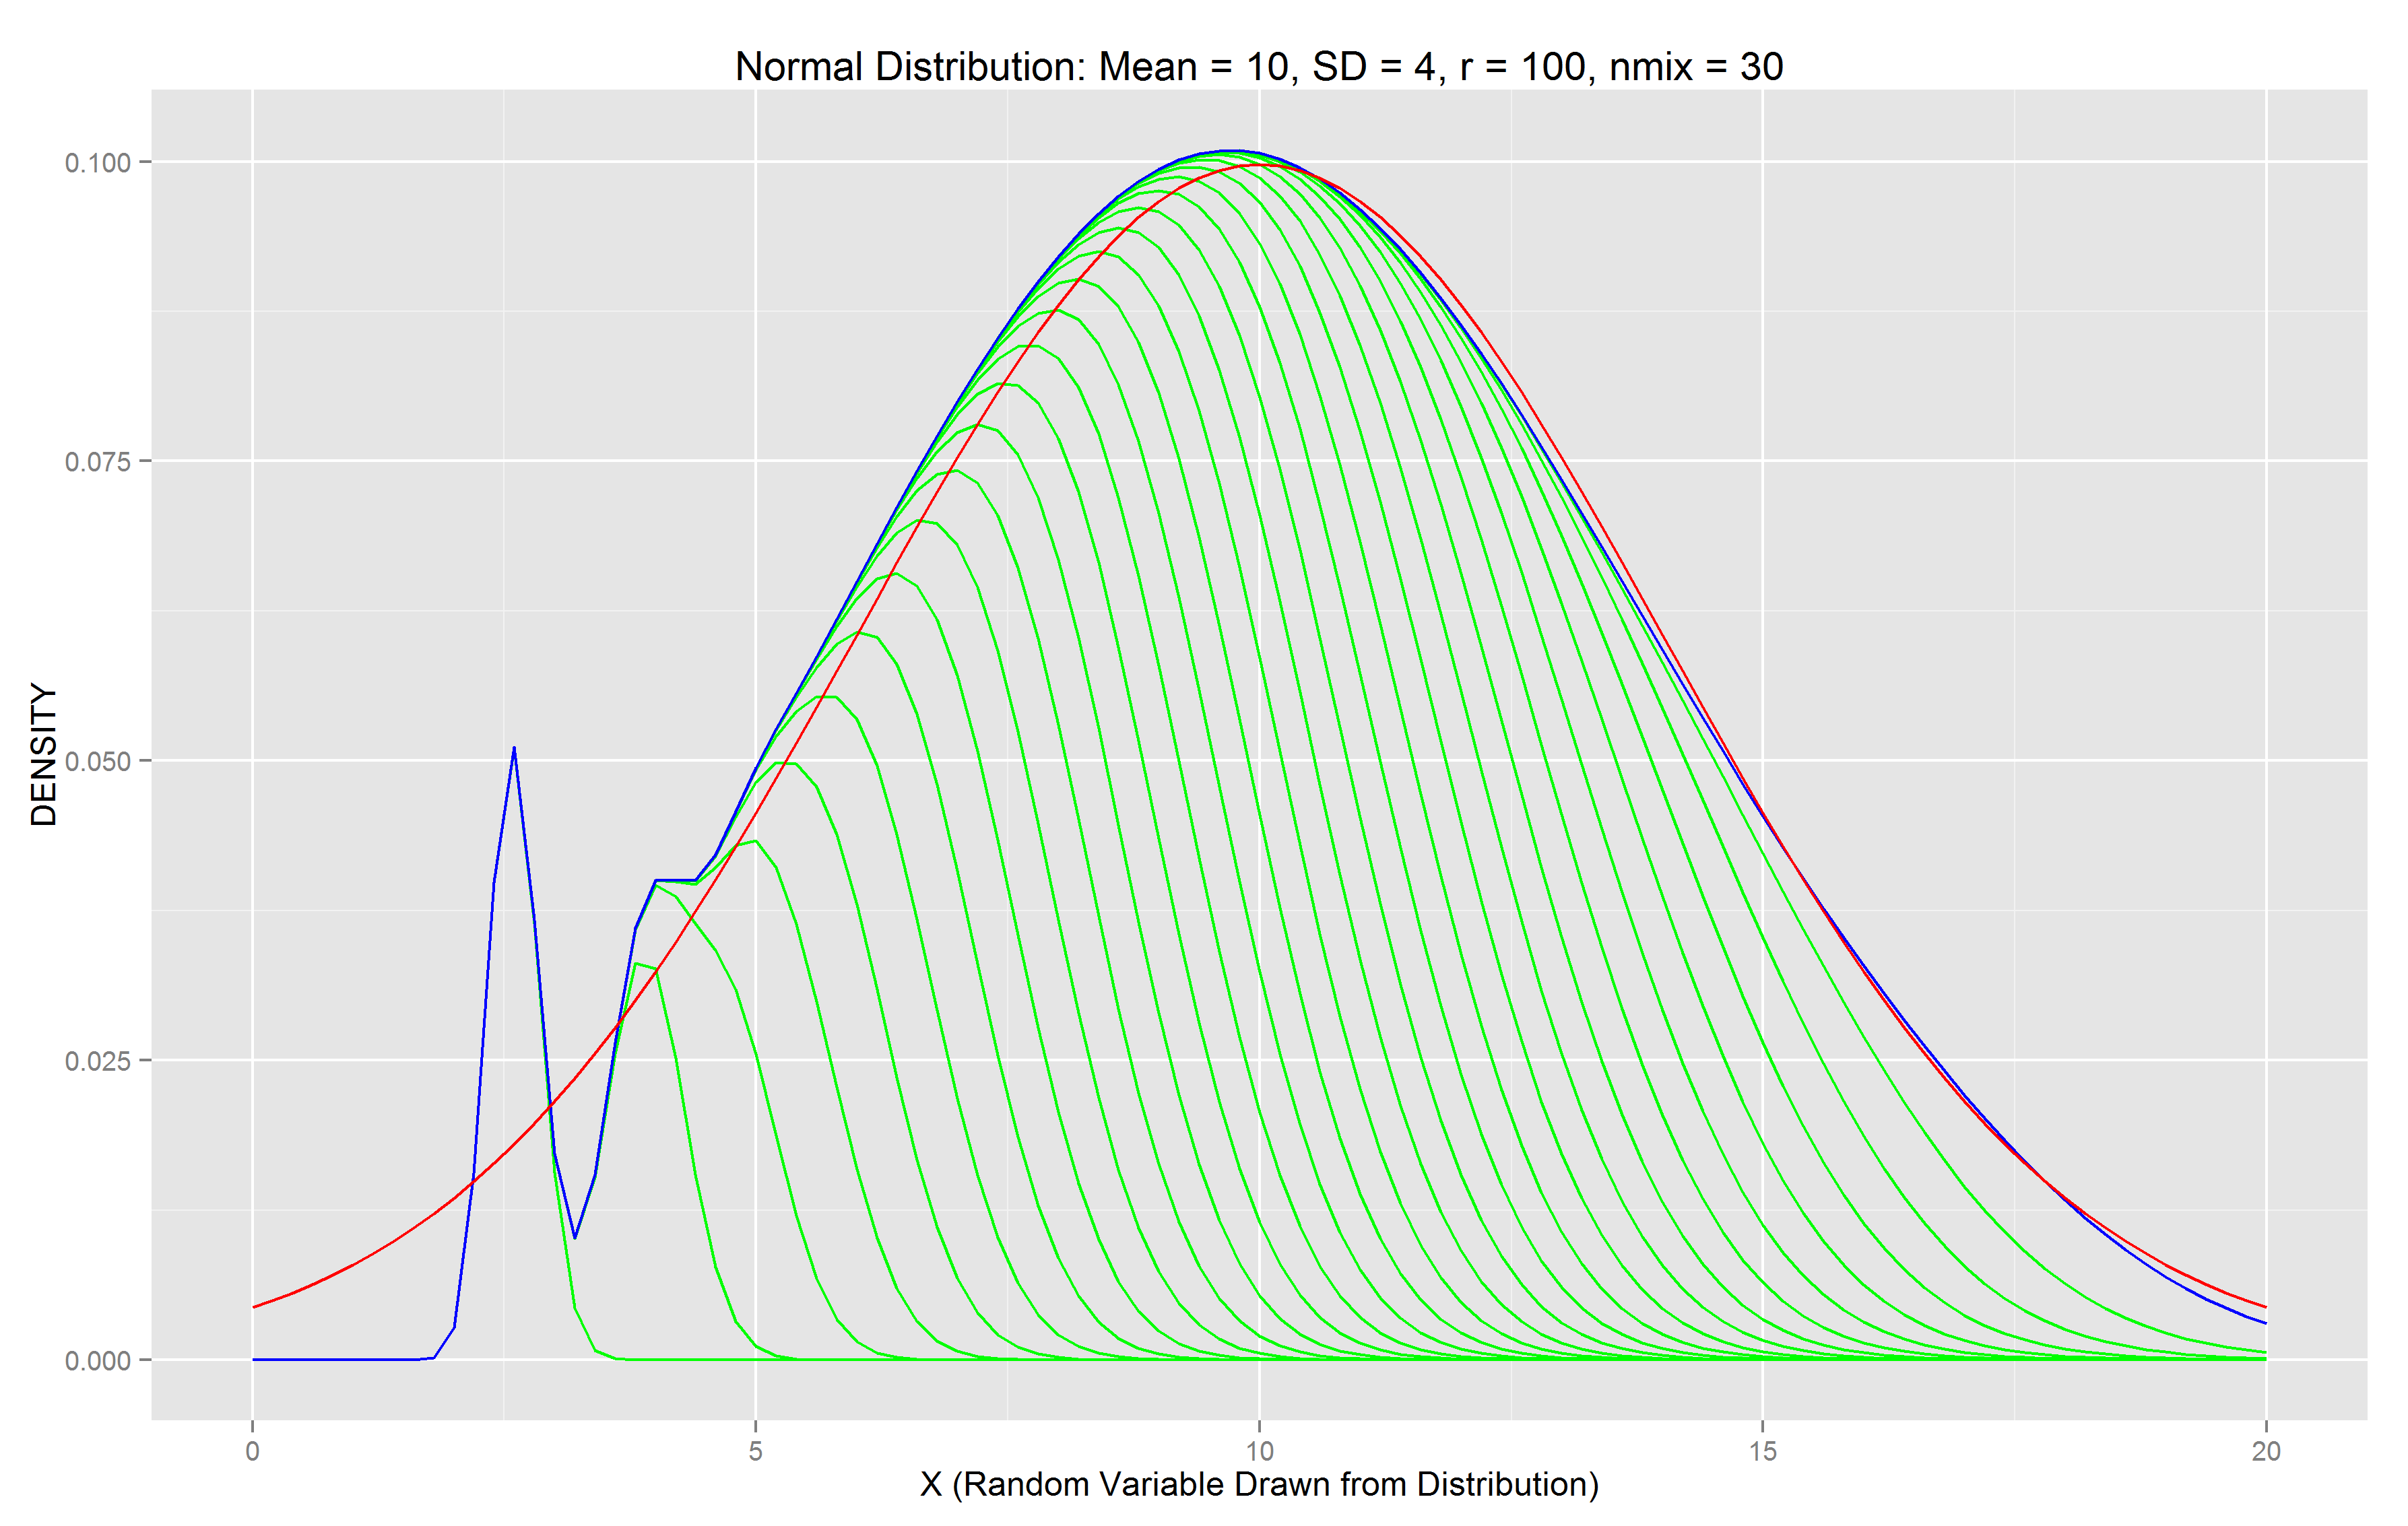
\includegraphics[scale=.27]{normdist_10_4_100_30.png}\\
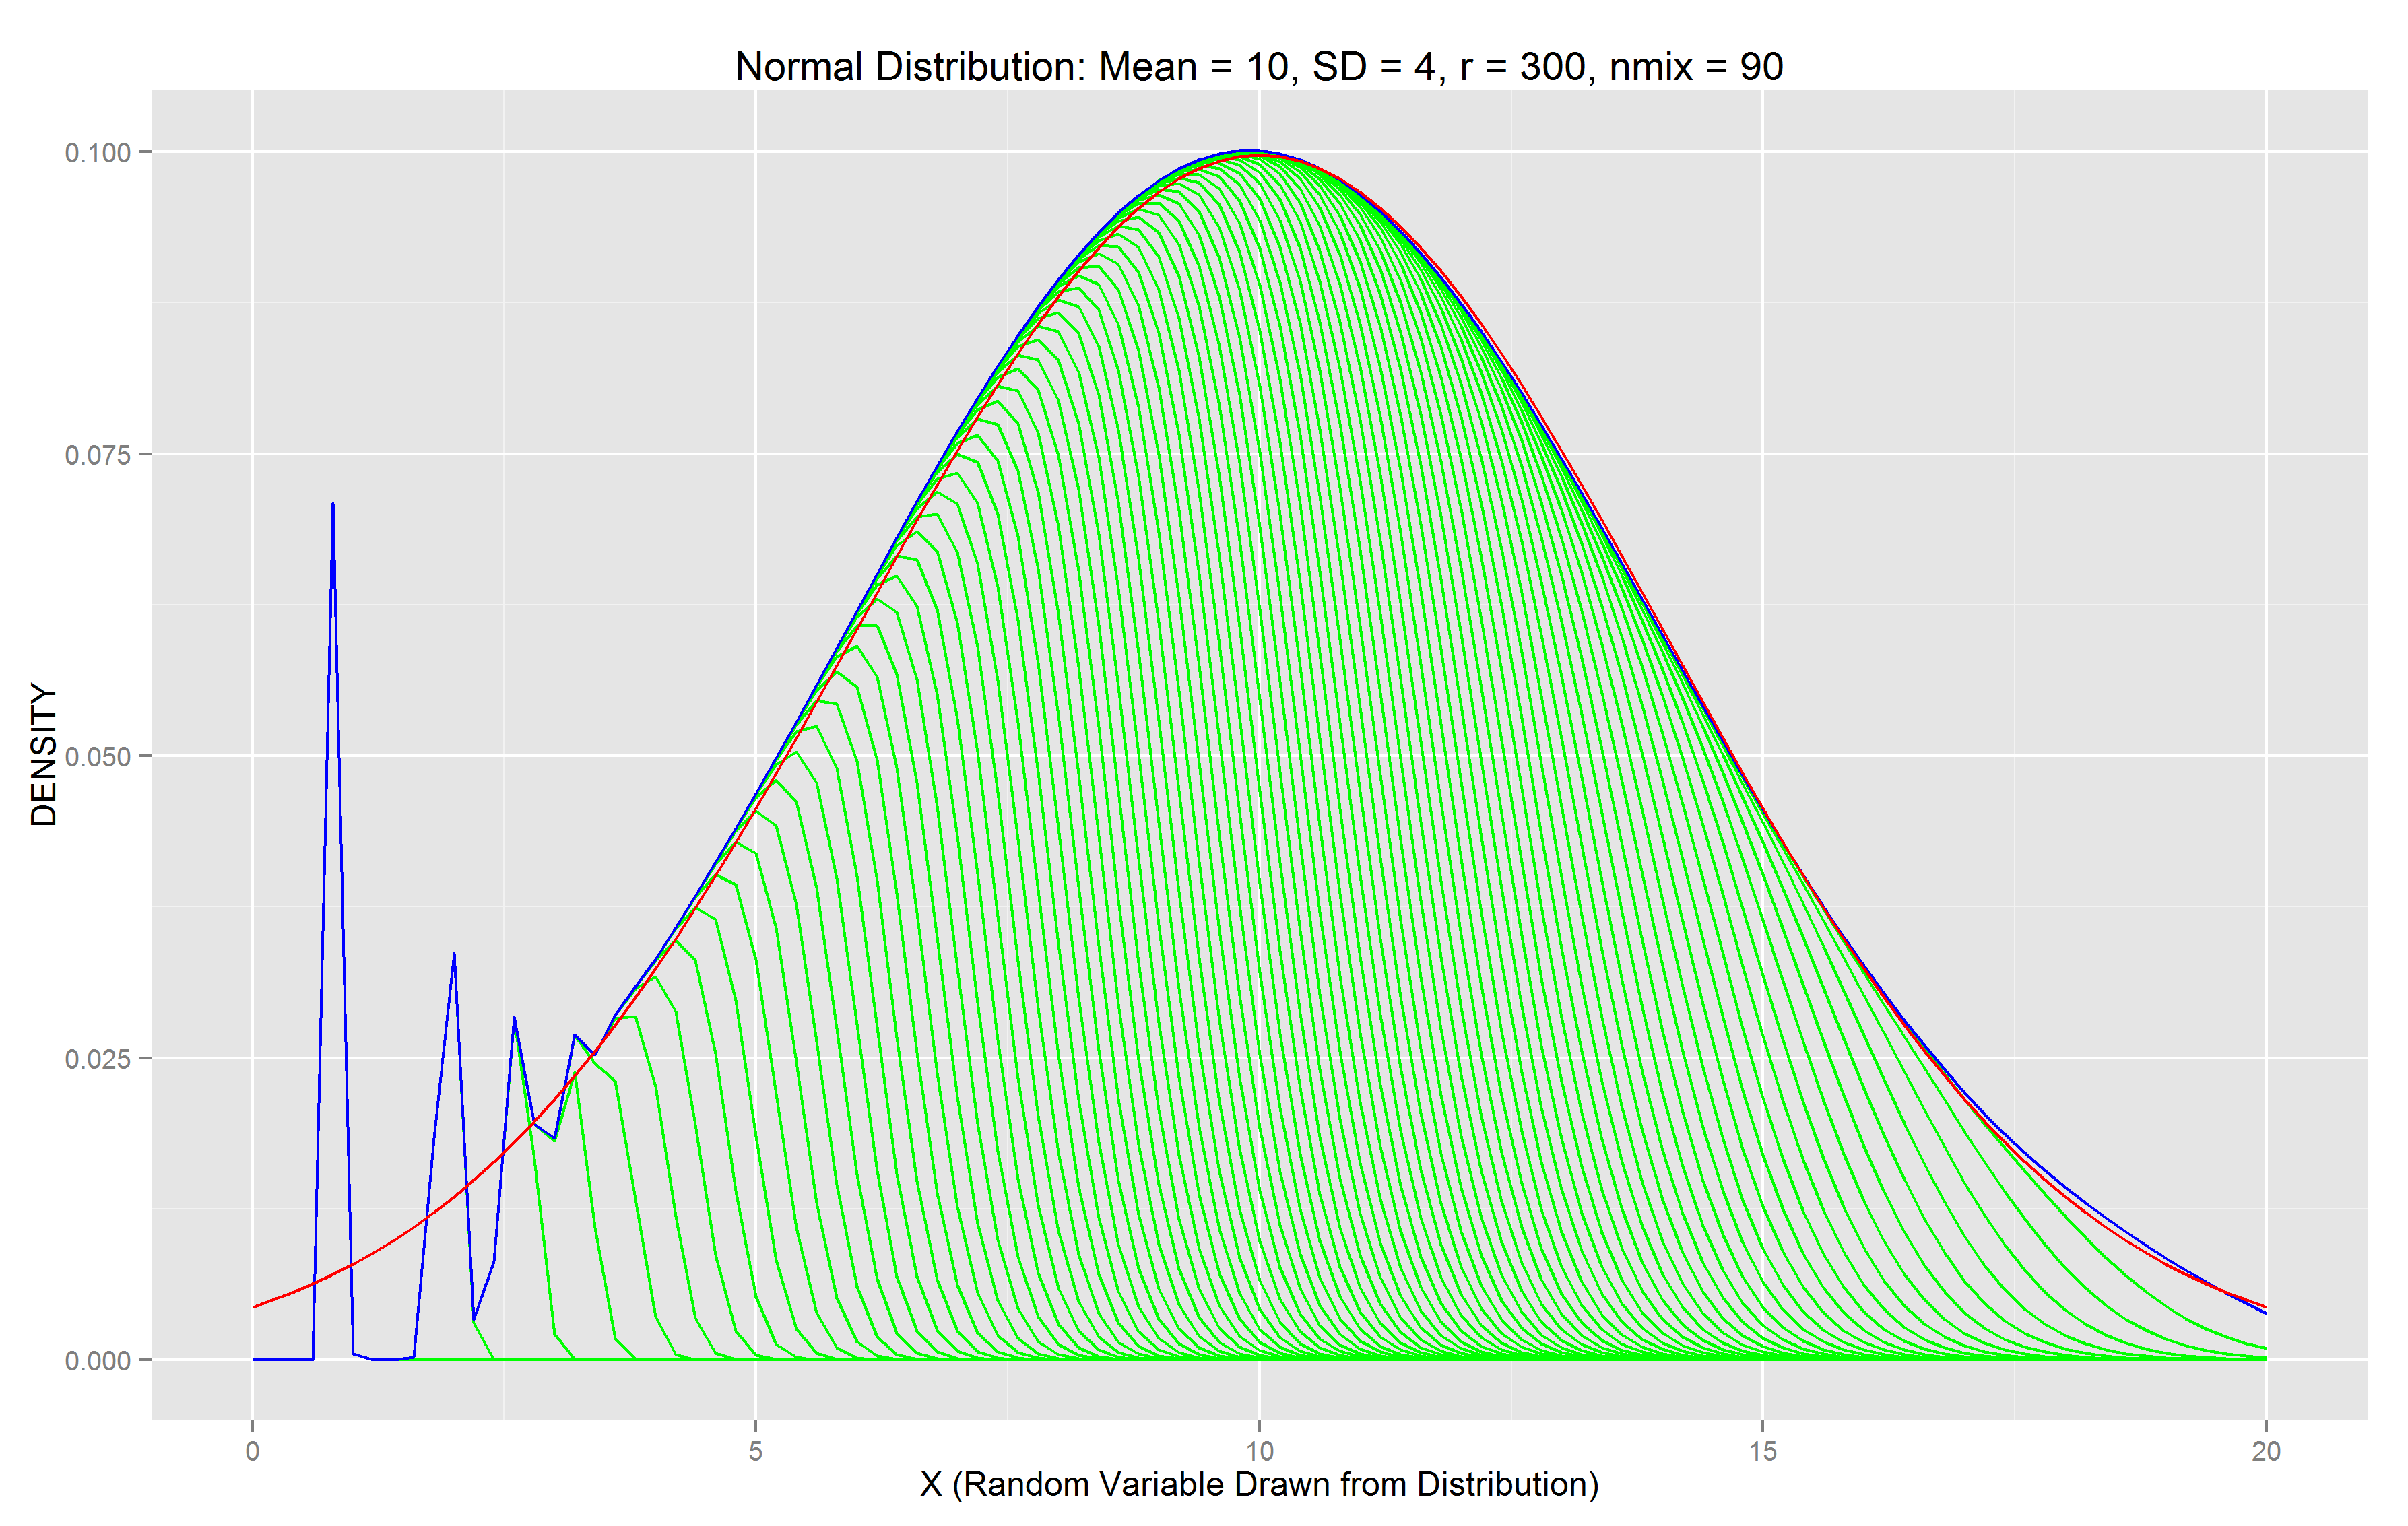
\includegraphics[scale=.54]{normdist_10_4_300_90.png}
\end{figure}

\newpage

As can be seen, as textbf{r} modifies the magnitude of each component within the approximation while textbf{nmix} controls the resolution of the approximation.  By increasing both, we can get an increasingly accurate approximation of the given distribution.

\subsection*{Problem 3.a}
See \texttt{HtoF.R}. 
\lstinputlisting{HtoF.R}


\subsection*{Problem 3.b}
Given a hazard function, $h(t)$, the density function, $f(t)$, can be found as follows:
\begin{equation*}
  \begin{aligned}
      f(t) = h(t) \cdot e^{-\int_0^t \mathrm{h(s)}\,\mathrm{d}s}
  \end{aligned}
\end{equation*}
We looked at the following hazard functions to explore what their density would look like:
\begin{equation*}
  \begin{aligned}
      h(t) &= 5 \\
      h(t) &= 2t \\
      h(t) &= 4 - 2t  \\
      h(t) &= (t-0.5)(t-1)(t-1.5)(t-2) + 0.1\\
  \end{aligned}
\end{equation*}
\begin{figure}[H]
\centering
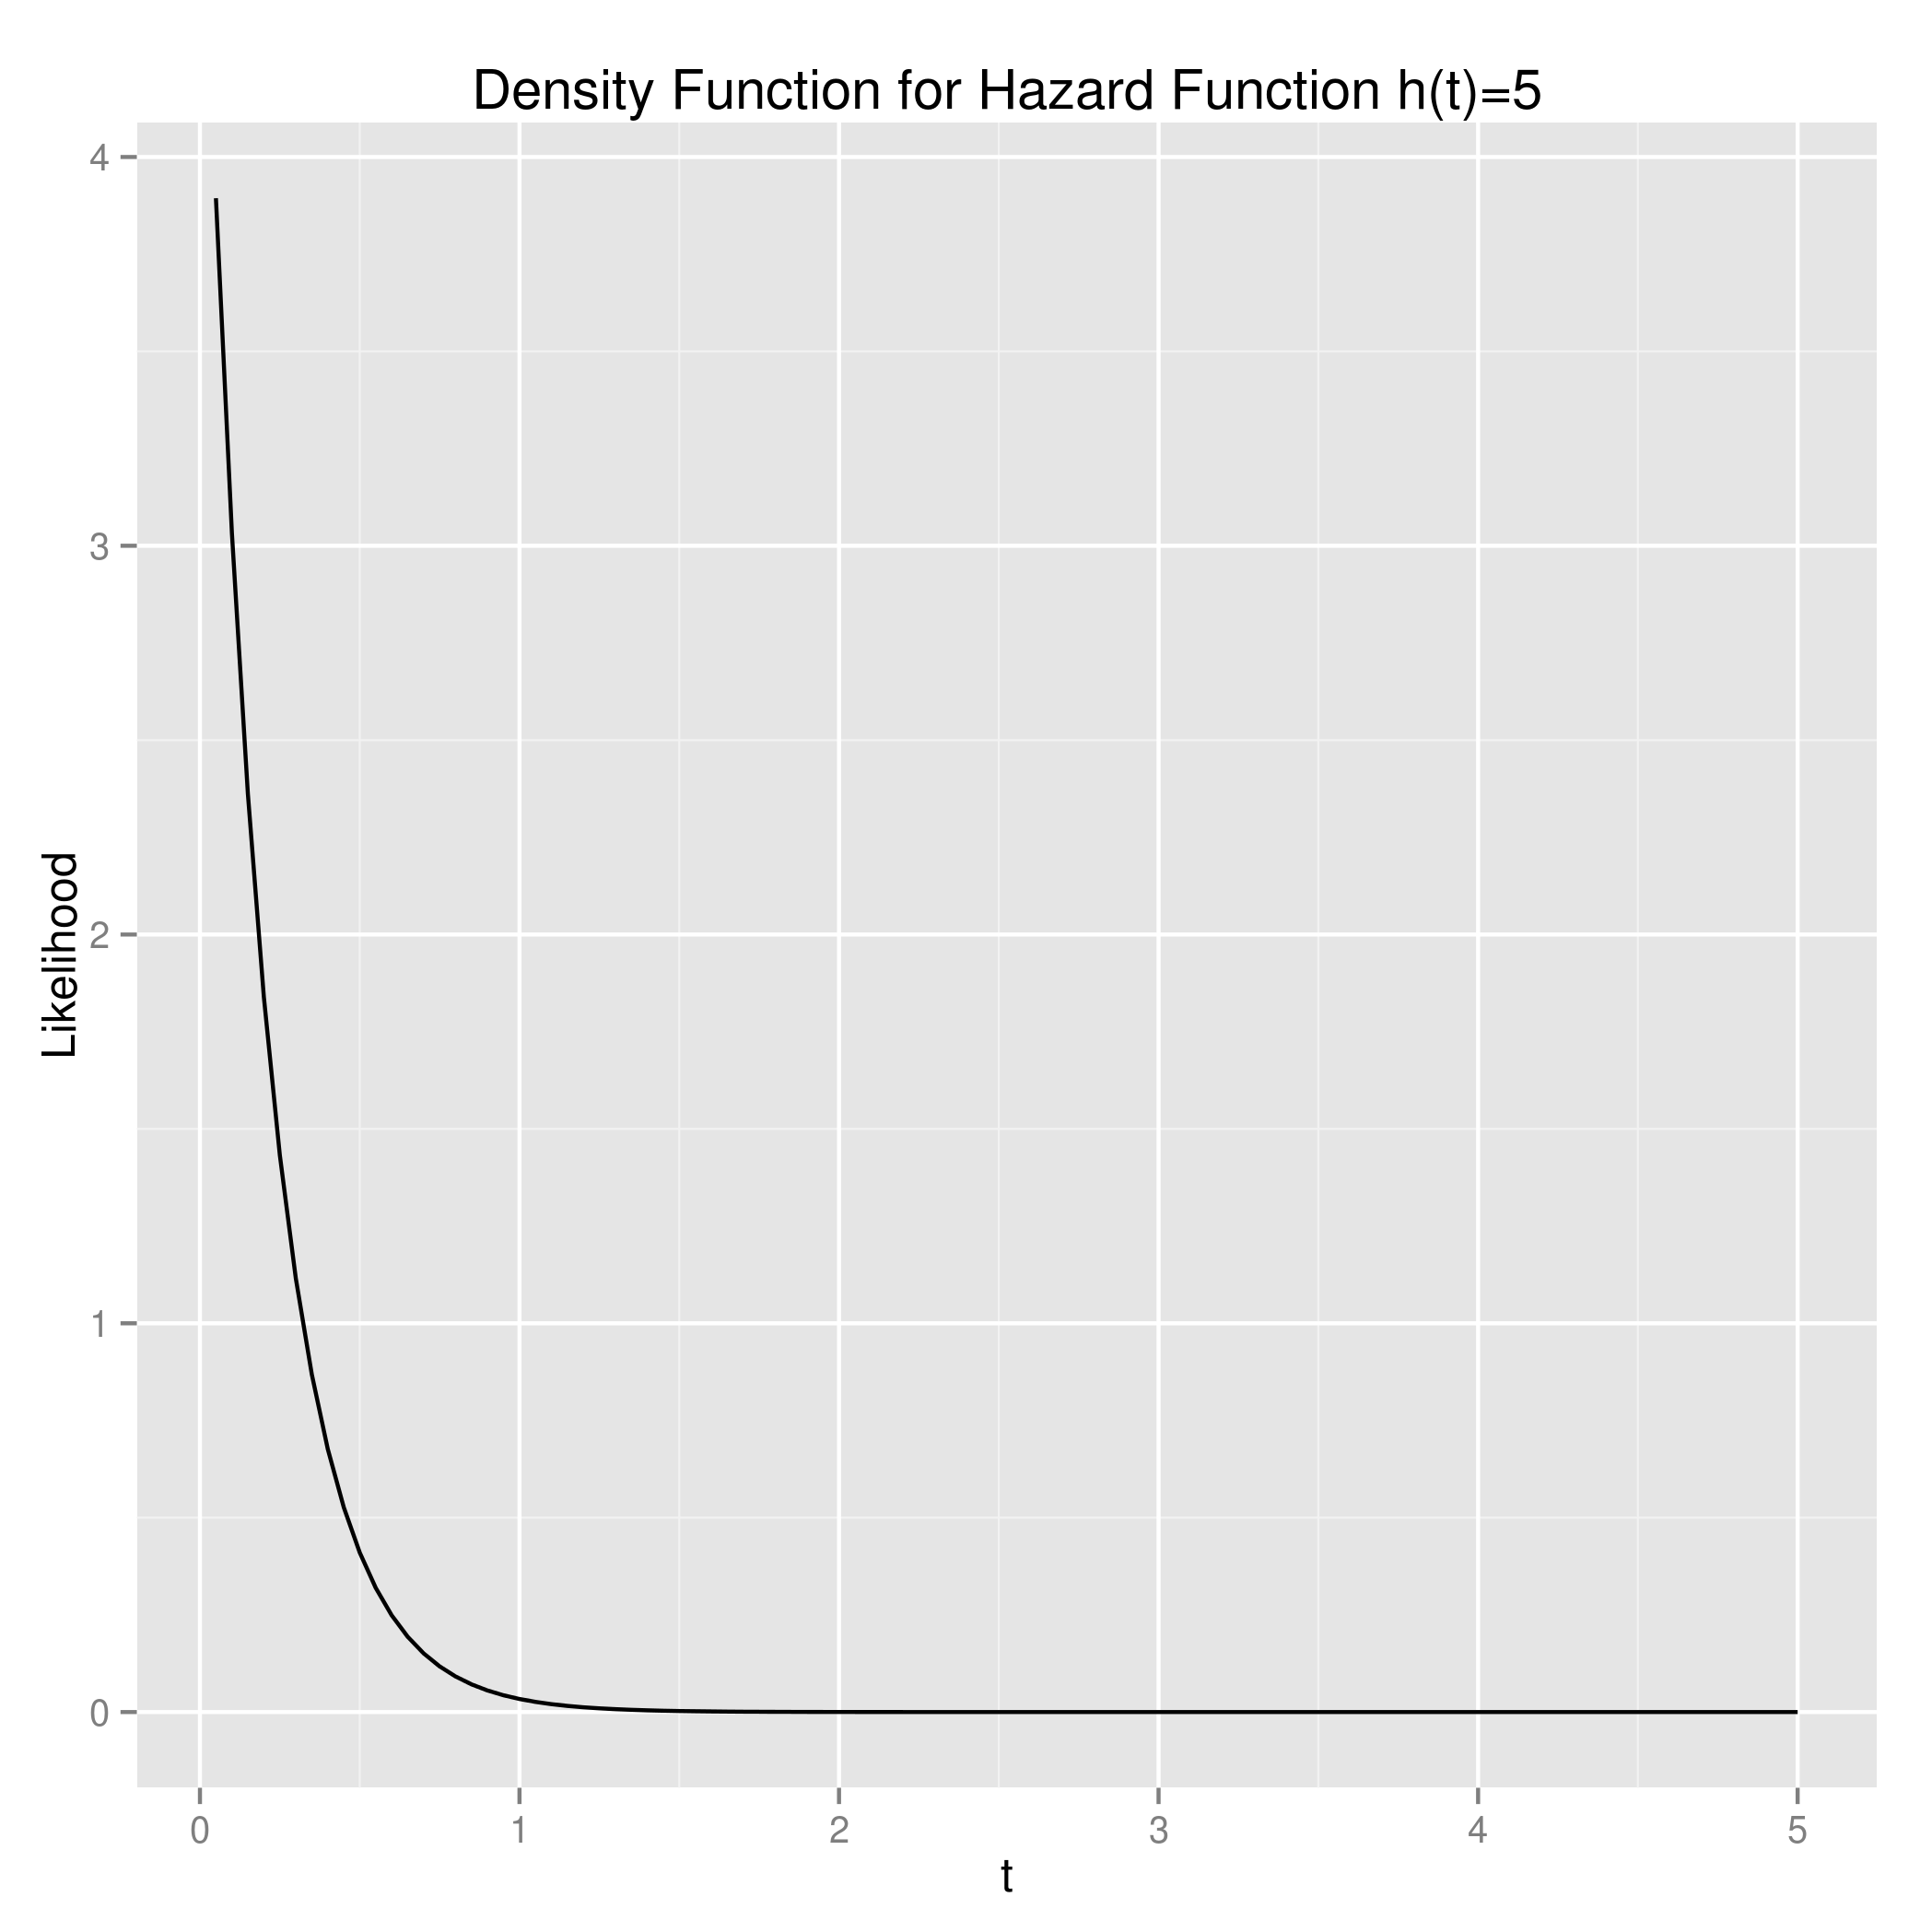
\includegraphics[scale=.33]{3_constant.png}
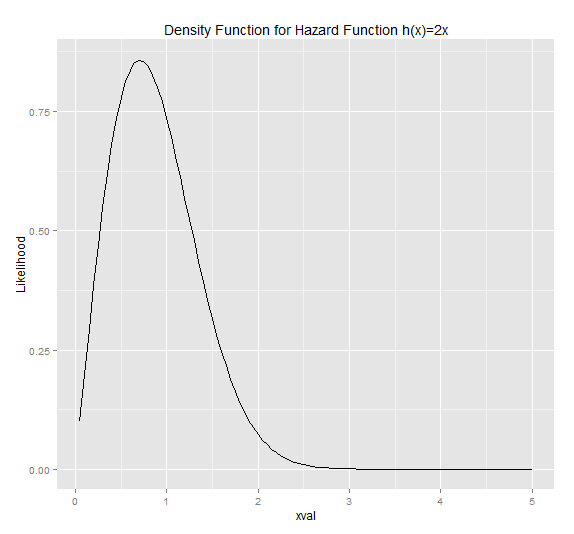
\includegraphics[scale=.33]{3_increasing.png}
\end{figure}
\begin{figure}[H]
\centering
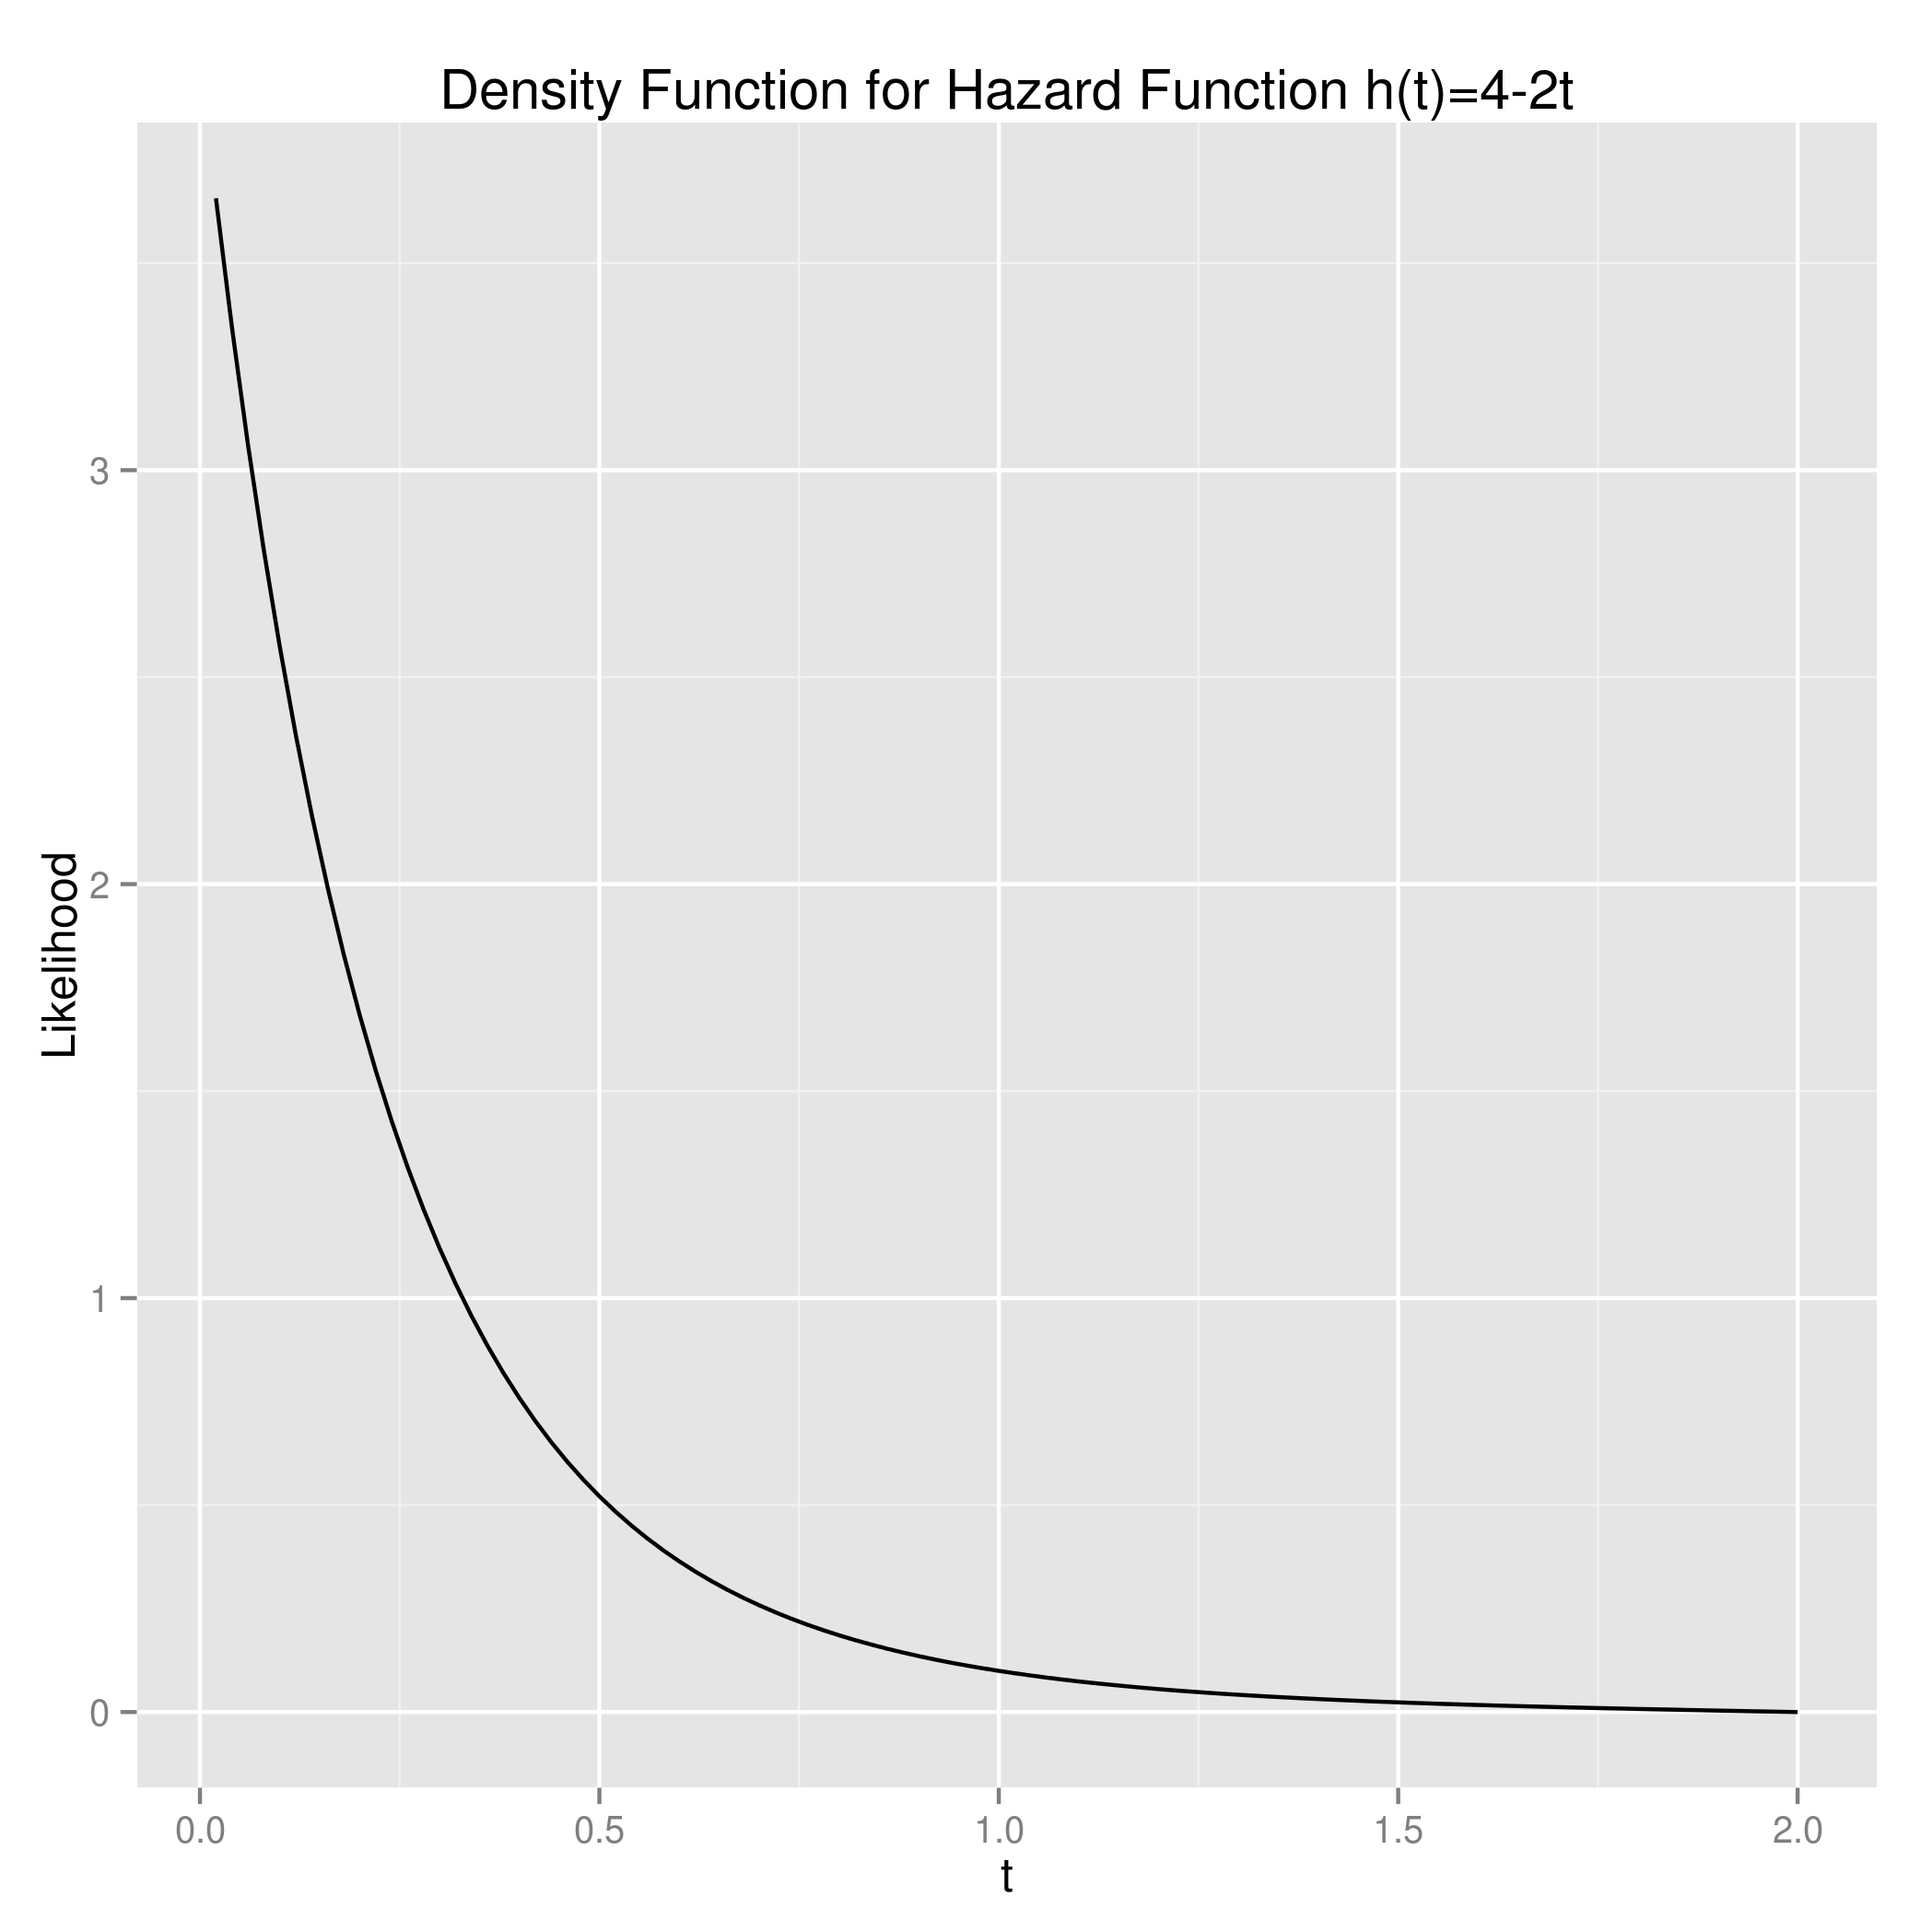
\includegraphics[scale=.33]{3_decreasing.png}
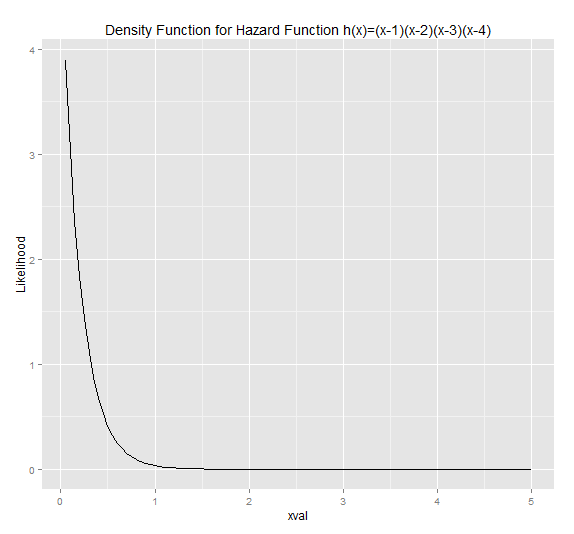
\includegraphics[scale=.33]{3_wshape.png}
\end{figure}
(Plots generated with \texttt{3.R}). 


\subsection*{Problem 4.a-b}

See \texttt{4.R} for generating these plots. 
\begin{figure}[h]
 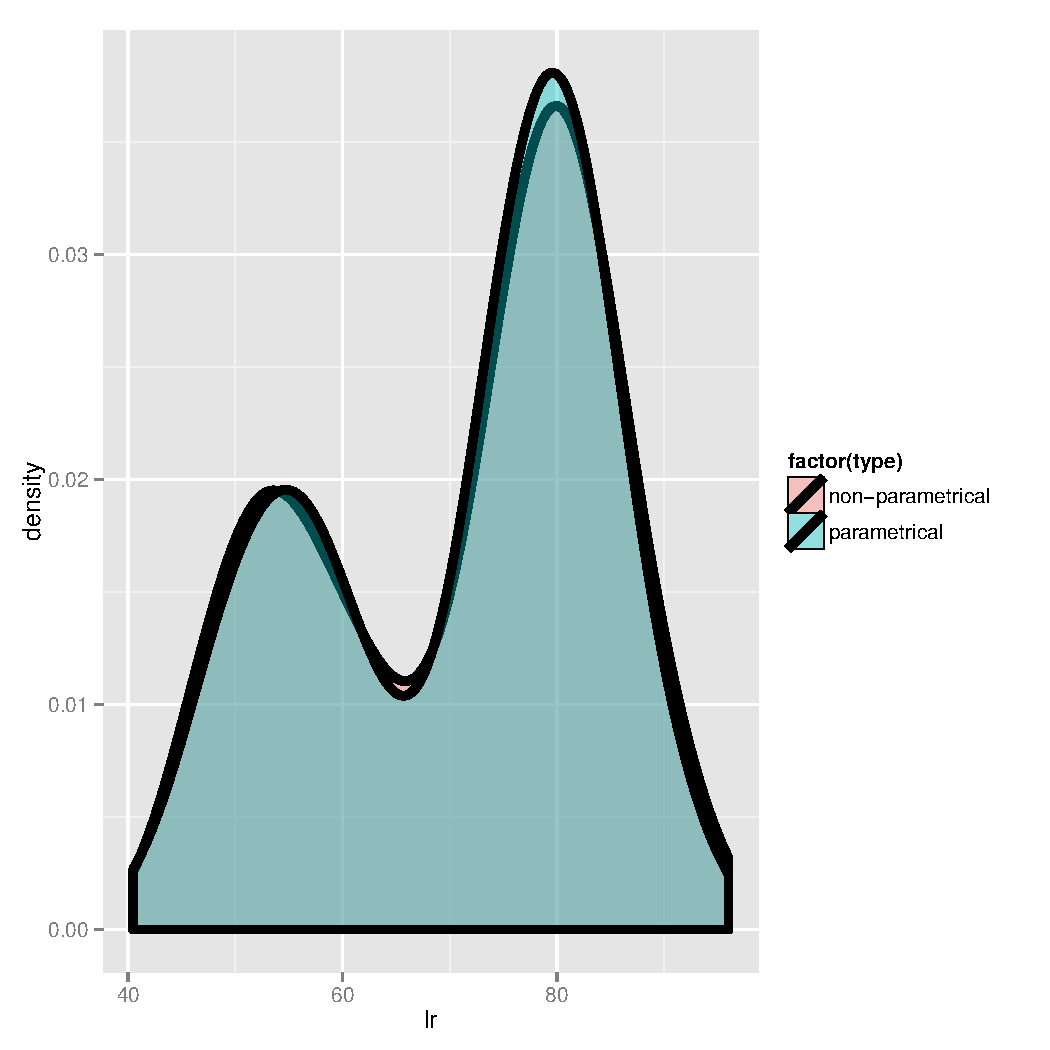
\includegraphics[scale=0.5]{plot4b.pdf}
\end{figure}
\pagebreak

\subsection*{4.f}

Creating the estimate using the function is simple. Our function outputs a sample of D, so to get an estimate of ED we simply take the mean of the sample outputted by our function. Doing this for simrenewal(10000, 20) gets us an estimated ED of [\textbf{BOX THIS ANSWER} 37.247 ].

The alternate estimate using Eq 11.31 is more complicated, and requires some derivation. Eq 11.31 is the following.

\begin{equation}
	ED = \frac{E(L^2)}{2EL}
\end{equation}

Where L is a random variable representing the lifetime. Now, we need to calculate $EL$ and $E(L^2)$, which we will do using the results of the EM analysis. The results from EM give us a mixture distribution of two normals, where it selects from normal $N_1(\mu_1, \sigma_1)$ with probability $p$ and $N_2(\mu_2, \sigma_2)$ with probability $p-1$. First, $EL$, using the law of total expectation. Here, we will use an indicator variable B, which will indicate which normal our mixture selected. So we'll say it's 1 with probability $p$, and 2 with probability $1-p$.

\begin{equation}
\begin{aligned}
	EL &= E(L | B) &=  	\begin{cases}
					E(N_1),  w.p. \; p \\
					E(N_2),  w.p. \;1-p
				\end{cases}  \\
	&&= E(N_1) * p + E(N_2) \\
	&&= mu_1 * p + mu_2 * p
\end{aligned}
\end{equation}

Since all of those values are parameters returned by the EM analysis, we're now done with $EL$. To find $E(L^2)$, we'll work from the variance of L using the rearrangement of (3.31) from the book

\begin{equation}
	E(L^2) = Var(L) + (EL)^2
\end{equation}

We already have $EL$ from earlier, so we just need the variance of L, which we'll do using the law of total variance with the same indicator variable B. To do this, we first need $E(L|B)$, which we already have, and $Var(L|B)$, which is quite similar to $E(L|B)$

\begin{equation}
\begin{aligned}
	Var(L | B) &=  	\begin{cases}
					Var(N_1),  w.p. \; p \\
					Var(N_2),  w.p. \;1-p
				\end{cases}  \\
		&=		\begin{cases}
					\sigma_1^2,  w.p. \; p \\
					\sigma_2^2,  w.p. \;1-p
				\end{cases}  \\
\end{aligned}
\end{equation}

Now we can continue with the law of total variance, and substitute into equation 4.3 from earlier.

\begin{equation}
\begin{aligned}
	E(L^2) &=  E[Var(L | B)] + Var[E(L|B)] + EL^2 \\
		&= \sigma_1^2 * p + \sigma_2^2 * (1-p) + E(E(L|B)^2) -  E(L|B)^2 + EL^2 \\
		&= \sigma_1^2 * p + \sigma_2^2 * (1-p) + mu_1^2 * p + mu_2^2 * (1-p) -  EL^2 + EL^2 \\
		&= \sigma_1^2 * p + \sigma_2^2 * (1-p) + mu_1^2 * p + mu_2^2 * (1-p)
\end{aligned}
\end{equation}

Now we have $E(L^2)$ in the form of the results of the EM analysis, and we can finally calculate an ED estimate using eq (11.31), which with the paramters returned from EM analysis gave us [\textbf{BOX THIS ANSWER} 36.747], a reasonably close estimate to our simulations estimate.


\end{document}
